\documentclass[zihao=5,a4paper,fontset=none]{ctexart}
\usepackage[a4paper,top=17mm,bottom=18mm,left=20mm,right=20mm]{geometry}
\usepackage{graphicx,float,booktabs,tabularx,array,amsmath,amssymb,xcolor,enumitem,fancyhdr,hyperref,listings}
\setmainfont{Times New Roman}
\setsansfont{Arial}
\setmonofont{Menlo}[Scale=0.88]
\setCJKmainfont{Songti SC}[AutoFakeSlant=0.167]
\setCJKsansfont{Hiragino Sans GB}[AutoFakeSlant=0.167]
\setCJKmonofont{Hiragino Sans GB}
\setlength{\parindent}{0pt}
\setlength{\parskip}{3.5pt}
\setlength{\headheight}{15pt}
\setlength{\tabcolsep}{4pt}
\setlength{\intextsep}{7pt}
\renewcommand{\arraystretch}{1.18}
\linespread{1.12}
\ctexset{section={format=\Large\bfseries\sffamily,beforeskip=5pt,afterskip=7pt},subsection={format=\normalsize\bfseries\sffamily,beforeskip=6pt,afterskip=3pt}}
\hypersetup{unicode=true,colorlinks=true,linkcolor=black,urlcolor=blue,pdftitle={20位10MS/s数字模块九个月任务书}}
\pagestyle{fancy}
\fancyhf{}
\fancyhead[L]{\small 20b10mtask｜硕士生数字任务书}
\fancyhead[R]{\small SKY130HD｜九个月}
\fancyfoot[C]{\small 第\thepage 页}
\renewcommand{\headrulewidth}{0.3pt}
\setlist{nosep,leftmargin=1.7em,topsep=3pt}
\lstset{basicstyle=\ttfamily\scriptsize,breaklines=true,columns=fullflexible}
\tolerance=2500
\emergencystretch=2em
\begin{document}
\begin{center}
{\LARGE\sffamily\bfseries 20位／10 MS/s SAR ADC数字模块}\par\vspace{3pt}
{\large\sffamily 九个月任务书与数字验收要求}\par\vspace{3pt}
{\small 2026年11月8日｜已有工程接手版｜定义任务，不新增签核结论}
\end{center}
% ----- begin md -----

\section{先明确你要完成的任务与spec}

\textbf{最终目标：面向180 nm BCD、20位／10 MS/s SAR ADC，参考ISSCC 2024 9.8及相关专利，结合北大VLSI 2025的CAAZ机制；本阶段采用SKY130HD完成数字线性化与噪声抑制模块的Python$\to$RTL$\to$GDS，交付效果图、可综合RTL及数字验收报告。}

前7节是执行任务、spec及签核要求；后面的技术说明沿多张原图解释电路动作、误差、数字算法和复现边界。

\textbf{速率约定：}10 MS/s指原始转换；当前CAAZ按非重叠两笔合成一笔，正常输出5 MS/s，20位码宽不变。最终配对输出若要求10 MS/s，需另定内部20 MS/s规格。

你接手的是已有工程。主线固定为``切片调度＋DEM~$\to$~dither~$\to$~CAAZ~$\to$~整体数字后端''。先确认现有成果可复现，再补接口和证据缺口；不从头重写已经对拍的模块。以下为要求，不能理解为已经完成。

\begin{table}[H]
\small
  \centering
  \begin{tabularx}{\linewidth}{>{\hsize=0.45\hsize\linewidth=\hsize\raggedright\arraybackslash}X>{\hsize=1.25\hsize\linewidth=\hsize\raggedright\arraybackslash}X>{\hsize=1.25\hsize\linewidth=\hsize\raggedright\arraybackslash}X>{\hsize=1.05\hsize\linewidth=\hsize\raggedright\arraybackslash}X}
    \toprule
    阶段 & 要求你完成的任务 & 必交内容 & 截止与通过条件 \\
    \midrule
    模块一 & 复用调度／DEM及LMS，明确行为合同，补MC和输入／状态覆盖 & 选片／使用统计、DEM$\times$LMS四组线性度及频谱、接口记录 & M2：电荷／码关系正确，指定条件效果及独立留出、逐事件对拍通过 \\
    模块二 & 沿用八片dither，完善等效注入／去扰、时序及端点策略 & 注入图、无LMS／冻结LMS开关对照、全幅拒绝／超窗图 & M5：同笔归属正确，余量问题有处理与验证依据 \\
    模块三 & 沿用CAAZ控制／配对与共享AZ样本模型，补参数及协作场景 & AZ时序、同带宽噪声对照、保持误差扫描、错绑负例 & M7：行为确认／保持模型明确，配对及联合整数结果一致 \\
    整体交付 & 冻结整体RTL，完成SKY130HD数字宏实现与验证 & GDS、网表、SDC、SPEF、综合／时序／物理报告及摘要清单 & M9：按第6节逐项验收；缺少项明确保留未完成 \\
    \bottomrule
  \end{tabularx}
\end{table}

\textbf{行为级验收边界：}理想开关、电荷守恒、固定失配、理想ADC2和样本域噪声可以验证本课题算法；不以完整器件开关或模拟瞬态为前提。数字接口和行为条件在M1--M2冻结，旧GDS结论另行验收。

\begin{table}[H]
\small
  \centering
  \begin{tabularx}{\linewidth}{>{\hsize=0.6\hsize\linewidth=\hsize\raggedright\arraybackslash}X>{\hsize=1.4\hsize\linewidth=\hsize\raggedright\arraybackslash}X}
    \toprule
    项目 & 已定基线／尚待冻结 \\
    \midrule
    速率与调度 & 原始10 MS/s；18片池，8片采集、8片转换、2片空闲；CAAZ非重叠配对5 MS/s \\
    码制与模型 & 前级9位、输出20位二补码；模型ADC2为12位offset-binary、输入折算$\pm$100 mV，RA增益／窗口在行为合同中明确，实际电路映射另记；码宽不代表ENOB \\
    时钟与接口 & 16拍／笔时目标160 MHz、6.25 ns；样本ID、8个有序片号、扰动及AZ代必须同笔；IO时序预算待冻结 \\
    随机与配置 & 种子独立、非零；采集按使能推进，stall保持；配置同笔冻结。权重与映射模式匹配，不兼容模式切换先暂停／清空并重载系数 \\
    算术与异常 & 沿用Q28整数重构及既有位宽／舍入合同；$k=c-U$，下溢拒绝；不得静默回绕、限幅或丢样 \\
    工艺与电压 & 当前数字库为SKY130HD；$\pm$5 V是模拟差分输入范围，不是标准单元逻辑输入电压；数字电压域单独约束 \\
    性能验收 & 必须报告20位LSB的INL／DNL、SNDR／SFDR及拒绝；约100 dB为讨论目标，条件与数值门槛由预算及模型MC冻结 \\
    \bottomrule
  \end{tabularx}
\end{table}


\clearpage
\section{接手基础与九个月路线}

\textbf{工作树快照：}分支20b10mtask，算法基线包含bef5654动态修复，既有物理包另绑定66b2e2e；本次基于aea7d1f接手说明继续核对。以下分别登记能复用的代码／证据及缺口，不要求学生重新实现已有模块。~\href{https://github.com/defineiocc02/20bit_SAR_ADC_Behaviour_Verification/tree/20b10mtask}{直接获取学生交付分支}，在仓库根目录执行说明中的命令。

\begin{figure}[H]
  \centering
  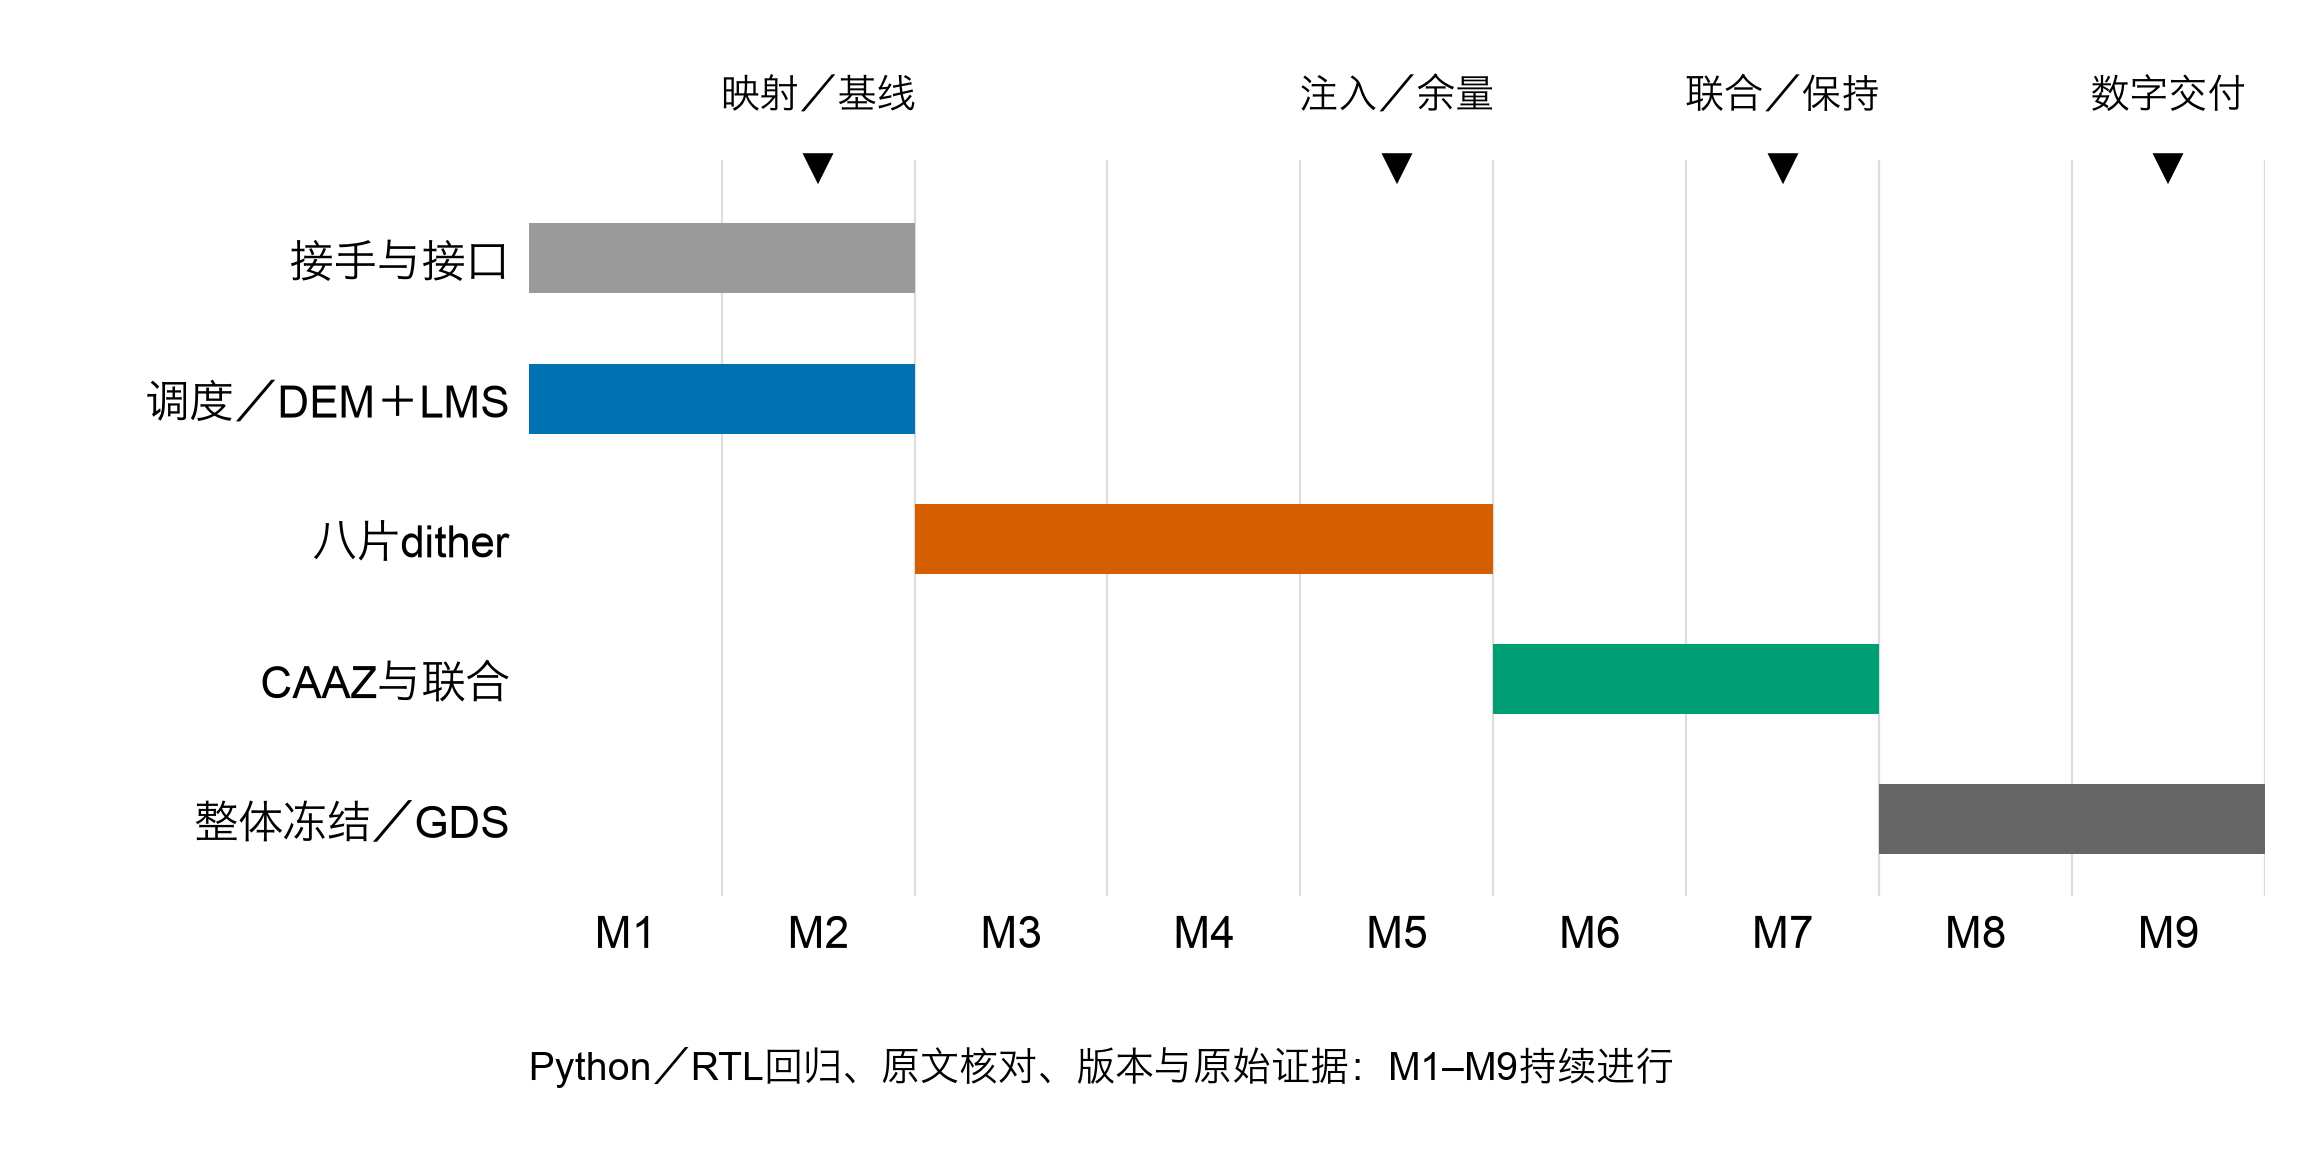
\includegraphics[width=146mm]{figures/nine_month_plan.png}
  \caption{九个月任务与阶段验收路线}
  \label{fig:九个月任务与阶段验收路线}
\end{figure}

首周只做``版本／环境检查＋已有数据回放抽查＋接口缺口登记''。已有图先原样引用并注明来源，需理解绘图口径时可重绘；无需重新训练、重新生成全量码密度或重做旧版图。接口、算法、条件或证据摘要改变后，才重跑受影响的完整验证。

\begin{table}[H]
\small
  \centering
  \begin{tabularx}{\linewidth}{>{\hsize=0.65\hsize\linewidth=\hsize\raggedright\arraybackslash}X>{\hsize=1.25\hsize\linewidth=\hsize\raggedright\arraybackslash}X>{\hsize=1.1\hsize\linewidth=\hsize\raggedright\arraybackslash}X}
    \toprule
    已有交付 & 证据确认到哪里 & 你还要补什么 \\
    \midrule
    调度、受限DEM及跨段候选 & 两份归档对拍零差异、源码匹配；本次20项测试和65,536组名义关系检查通过 & 核心电荷／码机制成立；按物理使用及效果补覆盖，不因逻辑相位分布要求重写DEM \\
    八片dither与重构 & 独立dither 20,000拍零差异；Q28重构已有16,384笔及4,096中点检查，对应记录源码一致 & 已有等效负注入可用于行为验证；补全幅端点和输入覆盖，解释浮点／整数差异 \\
    CAAZ与联合结果 & 数字控制／配对及共享AZ样本模型已有同带宽收益 & 补保持／增益、1/f或慢漂移样本场景及数字握手；模拟宏不是行为验收前提 \\
    整体数字路径 & 有归档PASS；两份整体记录的部分输入摘要与当前文件不一致 & 核对RTL／参数／向量，变化时定向重放；本次静态入口已重放一致，不重写模块或旧收据 \\
    动态模型 & 218项Python回归记录，含33项动态检查；结构／数学核及条件输入图已验证 & 作为可选系统敏感性研究；不覆盖或否定当前静态行为结果，局部128码不外推全幅 \\
    SKY130后端 & 冻结源码66b2e2e的两个控制顶层有GDS、TT提取后时序和独立物理记录 & 含片上重构的当前整体顶层仍需交付；多角、等价、电源完整性未由旧包证明 \\
    \bottomrule
  \end{tabularx}
\end{table}

身份核对涉及on\_chip记录的experiment.py及joint\_noise记录的summary.json摘要。本次行为静态入口、指标和训练均重放一致，未重跑RTL。数字发布前按RTL、参数、向量和约束的实际变化决定复验，不因文档依赖摘要变化无条件重做全部。

当前Python分为map\_fig11受限映射与map\_fig21\_bridge跨段候选，八片实验的fig21\_dem支路实际使用后者。其电荷等效及数字机制可进行行为验收，不要求先做MUX器件瞬态。代码复核还纠正了旧说明：Fig.11本来标有8C／4C／2C／C／C；主侧两个1C均可参与DEM，恒低的是子阵列dummy。~本次行为审计复算24组频谱、16组线性度、四组NLMS训练及CAAZ四组，均与原结果一致。结合实际物理组后，逻辑起点分布不均未显示明显的使用劣化，不能判为功能缺陷，也不列为必须先修项。


\clearpage
\section{M1--M2：切片调度、DEM与LMS}

\textbf{复用：}task1中的调度、DEM候选、RTL和测试，以及现有片外LMS与定点重构工具。\textbf{新增：}冻结行为模型中的可交换单元和跨段补偿，补独立统计与覆盖验证。原文依据为ISSCC 2024 9.8 Fig.9.8.1／3及US10511316B2 Fig.11、20、21。~已有DEM＋LMS线性度改善可作为有效行为基线。后续重点为多种子、输入覆盖与整数／RTL维护；逻辑相位、物理使用及最终性能分开评价，不把单一计数当算法缺陷。

\begin{figure}[H]
  \centering
  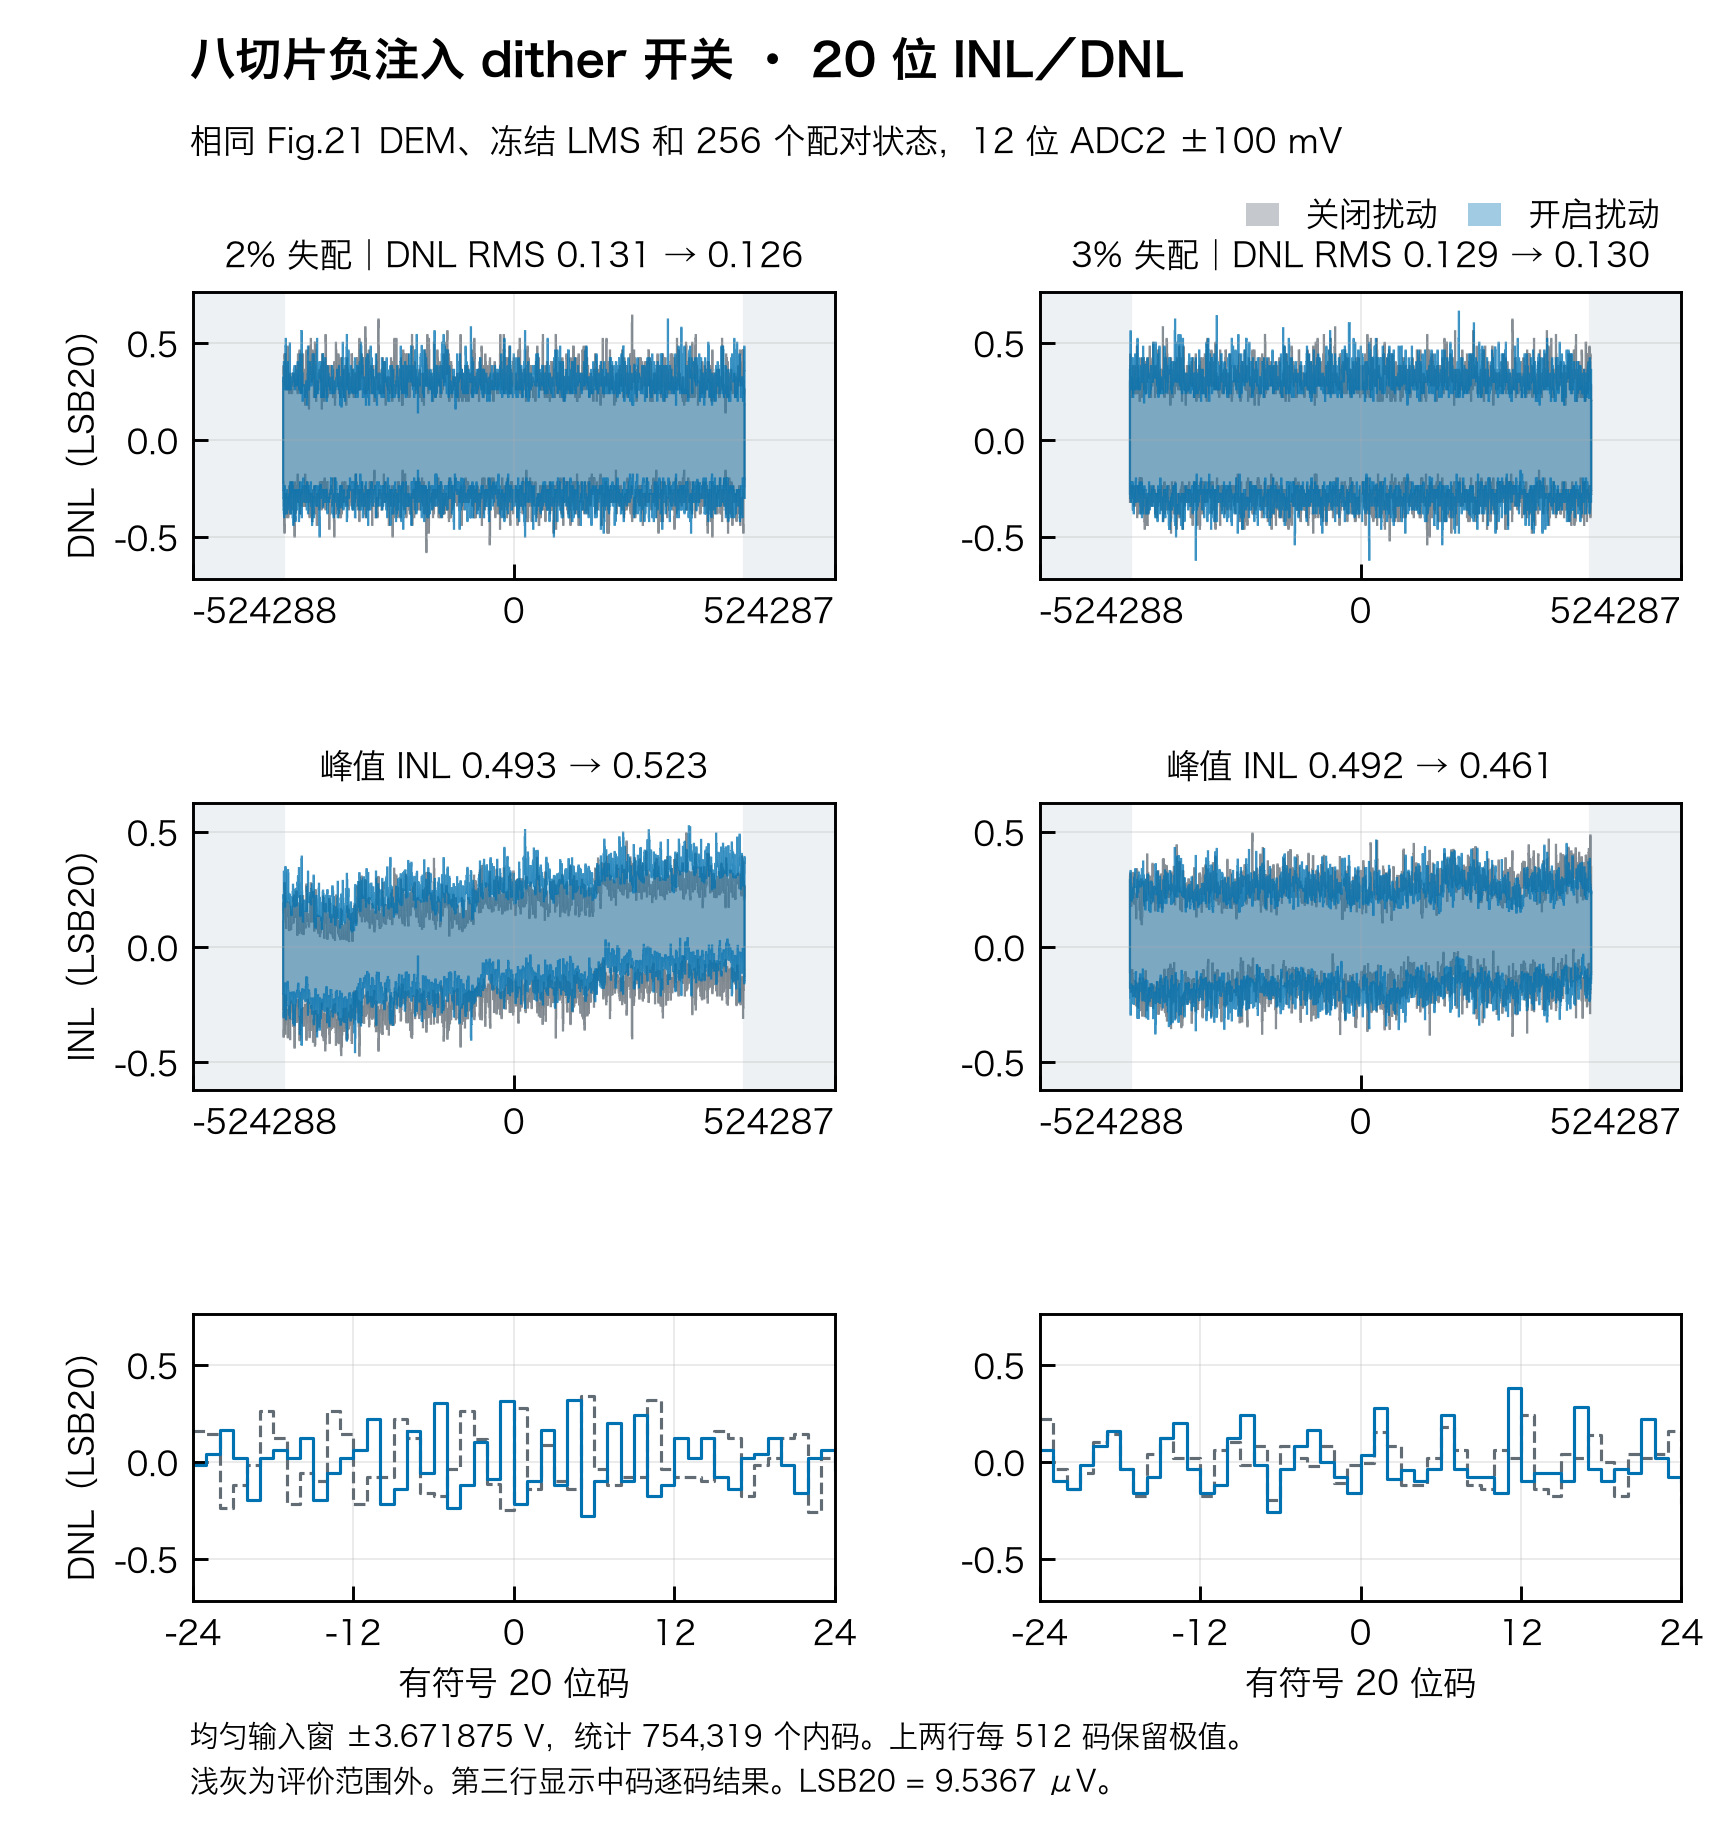
\includegraphics[width=125mm]{../task2/evidence/eight_negative/eight_native_linearity.png}
  \caption{已有静态线性度基线，供回放核对，不代表学生新增成果}
  \label{fig:已有静态线性度基线-供回放核对-不代表学生新增成果}
\end{figure}

已有2\%失配、dither关闭的峰值端点INL：无DEM／无LMS 655.668、仅LMS 0.788、DEM＋LMS 0.493 LSB20。条件为$\pm$3.671875 V共同窗、256个等权配对状态；不等于全幅单次无缺码。

\begin{table}[H]
\small
  \centering
  \begin{tabularx}{\linewidth}{>{\hsize=0.6\hsize\linewidth=\hsize\raggedright\arraybackslash}X>{\hsize=1.4\hsize\linewidth=\hsize\raggedright\arraybackslash}X}
    \toprule
    必交图 & 怎样比较与验收 \\
    \midrule
    选片时序＋单元使用分布 & 标出18／8／8／2、样本晋升和stall；转换组等于上一采集组，使用统计注明分母 \\
    DEM$\times$LMS四组20位INL／DNL与频谱 & 固定同一电容池、输入与可比控制，2\%／3\%分别报告；不能只给未校准图 \\
    训练收敛及冻结／留出 & 标明训练结束、冻结点、参考来源和独立验证；禁止用真实电容值充当已知校准系数 \\
    \bottomrule
  \end{tabularx}
\end{table}

通过条件：独立电荷关系正确、同笔掩码与配置稳定、Python／RTL整数对拍零差异。发生收益不足时报告原因与代价，不挑种子或缩窗后宣称达标。


\clearpage
\section{M3--M5：八片dither及内部余量}

\textbf{复用：}六位字发生器、八片注入模型、$k=c-U$命令、conv\_sub+sample\_sub重构及独立测试。\textbf{新增：}完善已声明等效电荷模型的端点与时序，扩大输入／失配覆盖。依据为ISSCC论文1页、讲稿17--18页及US10505561B2 Fig.3／19；专利七片示例与本工程八片分配分开标注。

\begin{figure}[H]
  \centering
  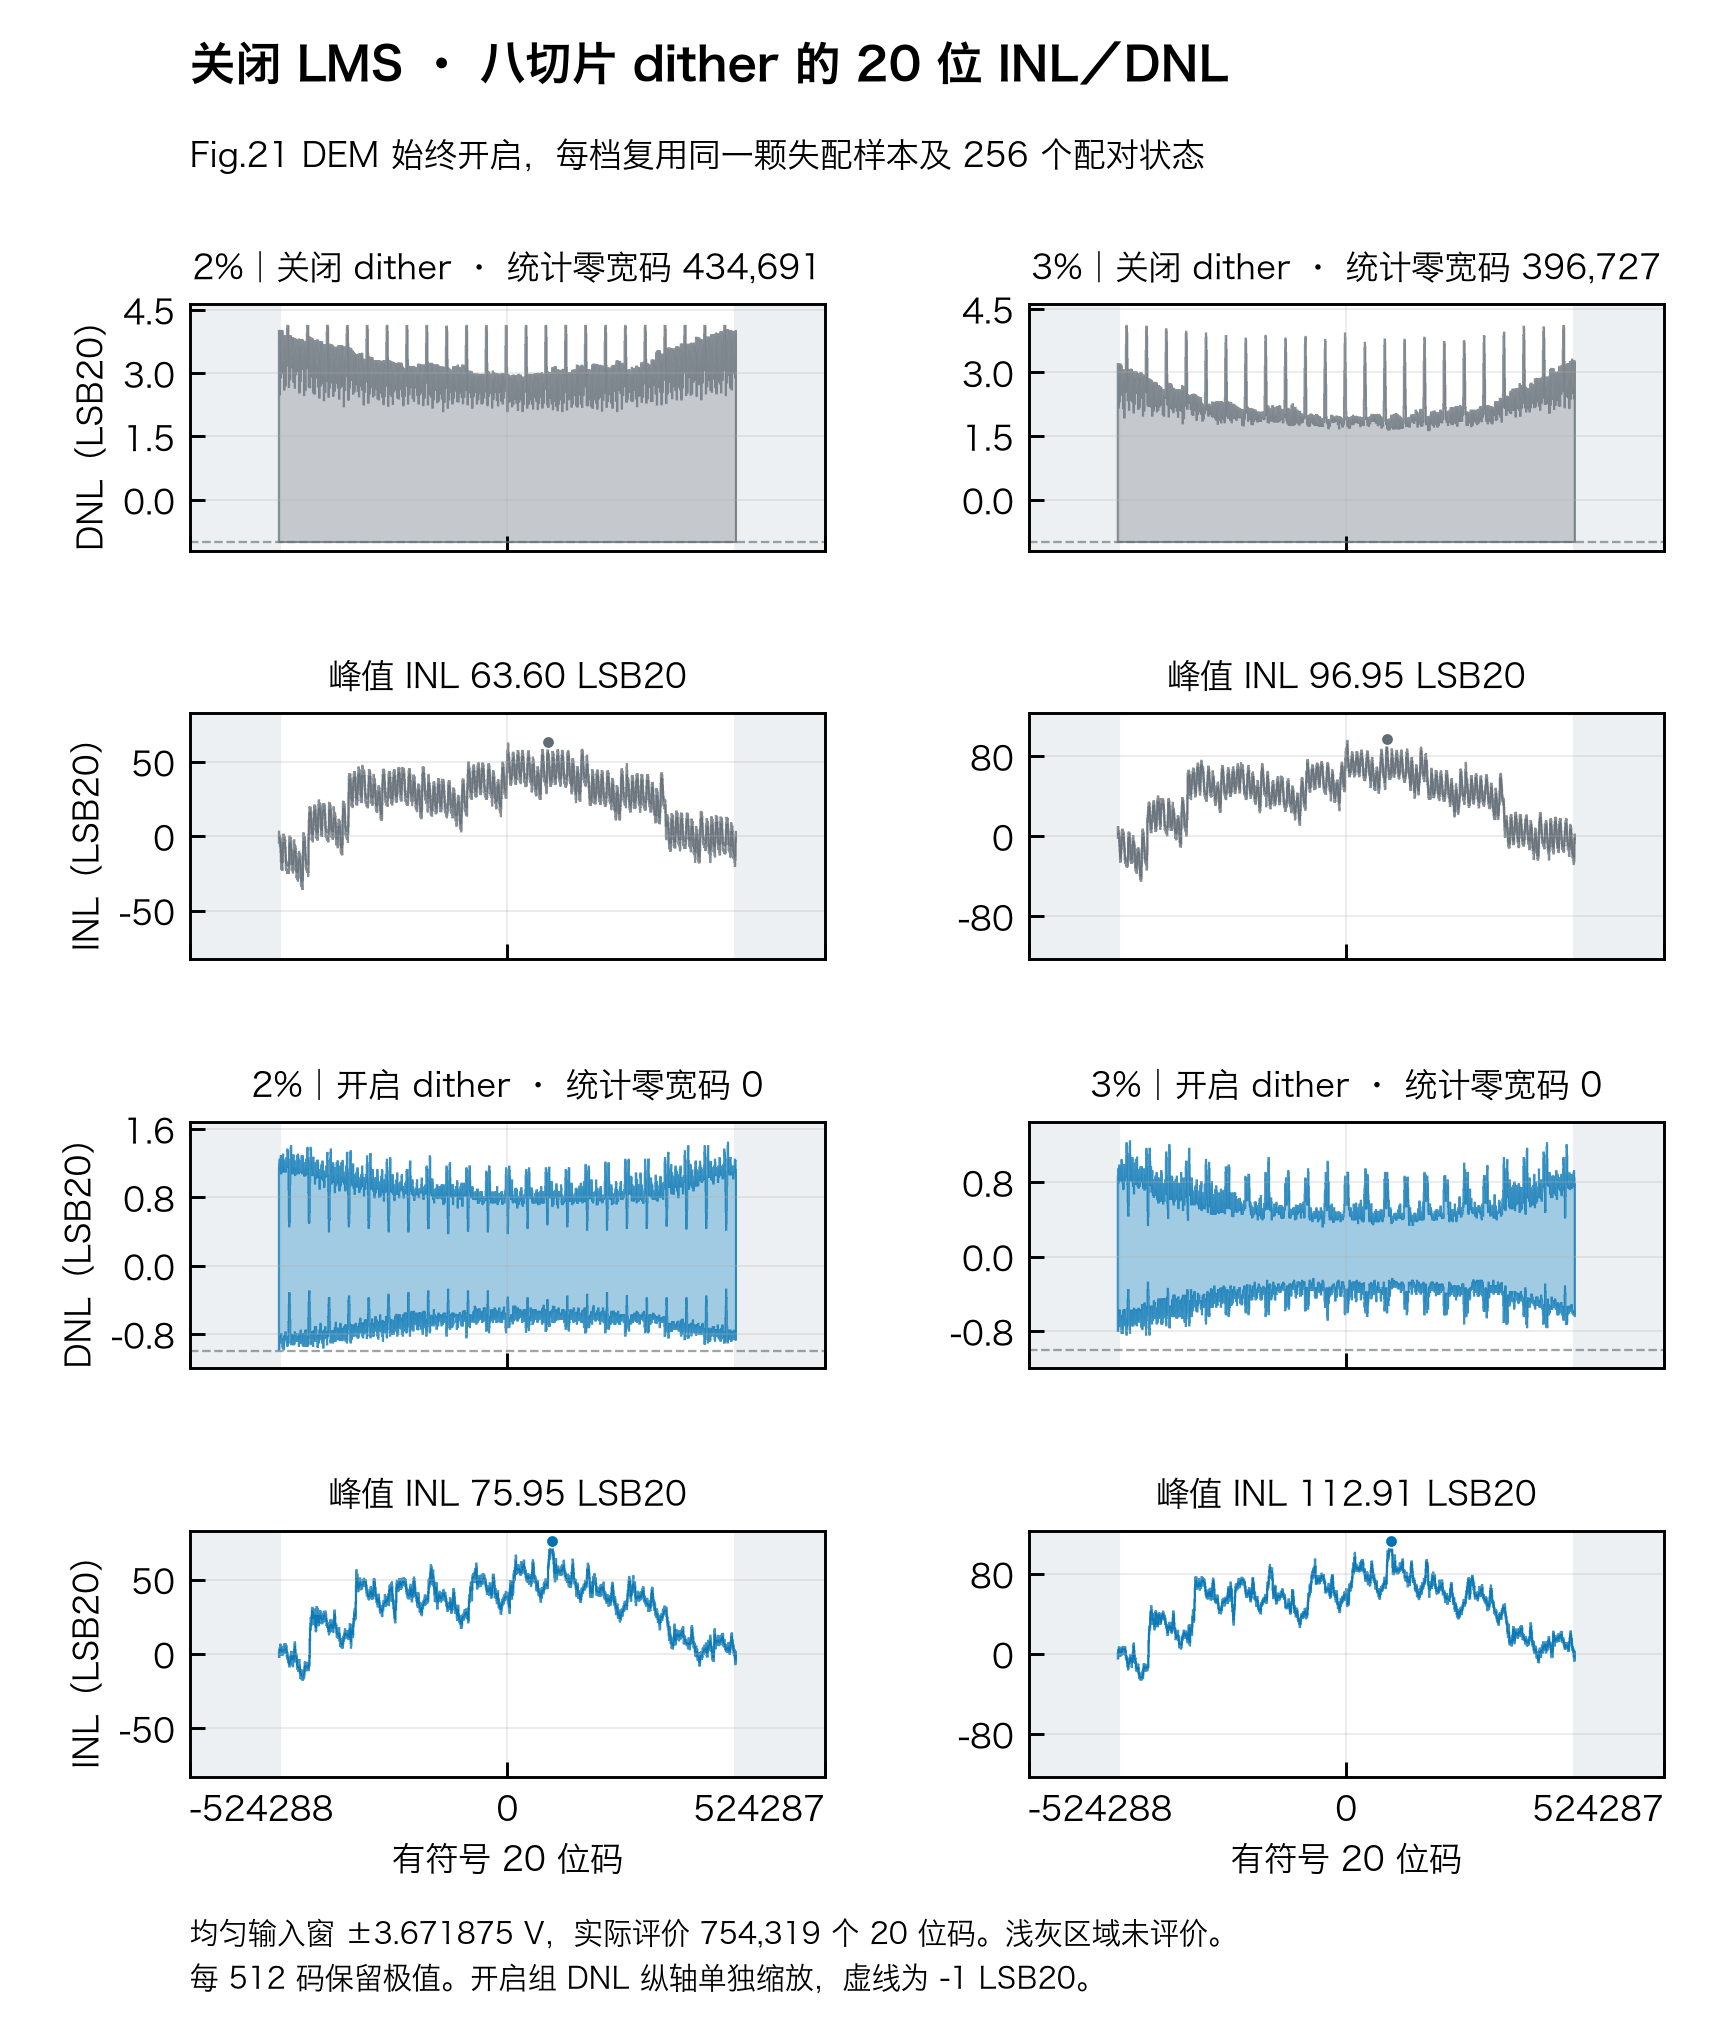
\includegraphics[width=119mm]{../task2/evidence/eight_negative/eight_native_no_lms_linearity.png}
  \caption{已有关闭LMS的dither对照，说明收益与代价需要同时报告}
  \label{fig:已有关闭lms的dither对照-说明收益与代价需要同时报告}
\end{figure}

已有DEM开、LMS关的2\%／3\%静态例中，零宽内码由434,691／396,727降为0，但峰值INL增大。当前全部字共同名义下限--4.855239 V，目标$\pm$5 V端点问题尚未闭合。图是平均码密度，不是实际模拟开关验收。

\begin{table}[H]
\small
  \centering
  \begin{tabularx}{\linewidth}{>{\hsize=0.6\hsize\linewidth=\hsize\raggedright\arraybackslash}X>{\hsize=1.4\hsize\linewidth=\hsize\raggedright\arraybackslash}X}
    \toprule
    必交图 & 怎样比较与验收 \\
    \midrule
    注入／去扰＋同笔时序 & 画出lower／upper、孔径、实际开关位图和数字补偿；逐项对照原文与工程选择 \\
    无LMS、冻结LMS各自的dither关／开INL／DNL与频谱 & 固定DEM、输入、失配池及训练合同；保留一个不使用LMS的独立对照 \\
    $\pm$5 V输入的拒绝／ADC2超窗与内部节点图 & 分开标前级拒绝、后级越界及最终码；不能靠数字限幅恢复已经过载的样本 \\
    \bottomrule
  \end{tabularx}
\end{table}

通过条件：同笔字／片号／掩码／ADC2对齐，独立整数与RTL一致；行为级余量与端点处理有依据；无需器件开关仿真才能认可该结果，实际芯片预测另行验证。


\clearpage
\section{M6--M7：CAAZ与三技术协作}

\textbf{复用：}斩波相位、带ID的AZ请求／确认、两笔配对和现有联合噪声实验。\textbf{新增：}在样本域扫描保持／两相增益及相关噪声，验证异常和联合数字行为。依据为Wang等VLSI 2025 C32-1 Fig.5／6；不要求学生设计RA或CBIAS模拟宏。

\begin{figure}[H]
  \centering
  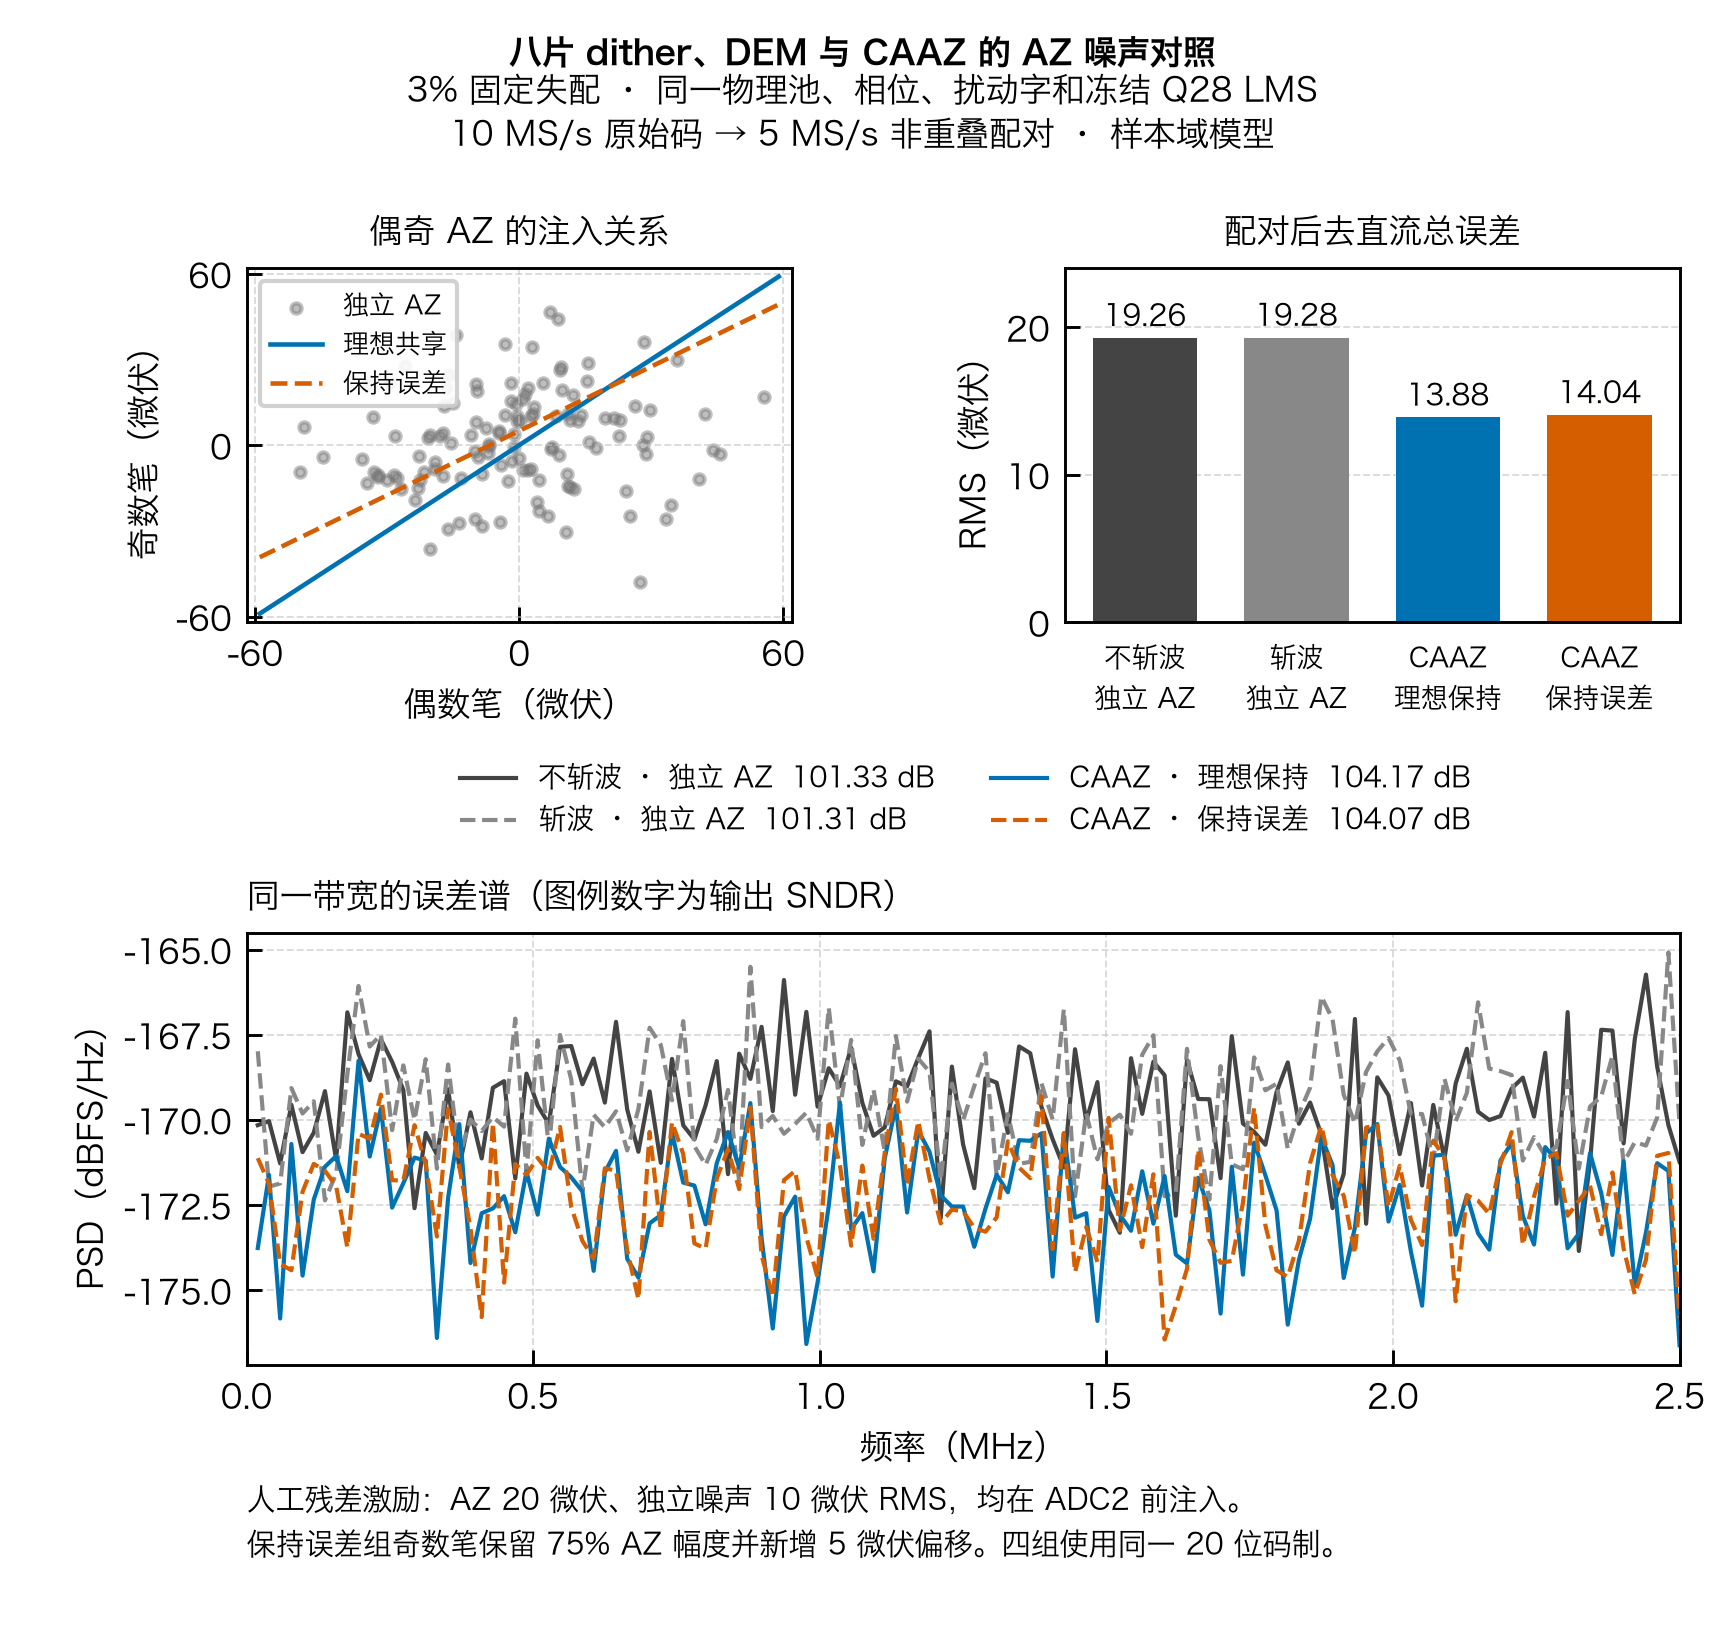
\includegraphics[width=125mm]{../task3/evidence/negative/joint_noise/caaz_joint_noise.png}
  \caption{已有声明噪声条件下的CAAZ效果，供核对等带宽比较方法}
  \label{fig:已有声明噪声条件下的caaz效果-供核对等带宽比较方法}
\end{figure}

已有同为5 MS/s输出的交流误差19.264$\to$13.875~μV RMS，加入示例保持误差后14.041~μV RMS。噪声及保持值为工程设置，不是真实电路测量。两点配对改变频响，不能把降低输出速率本身的收益归给CAAZ。

\begin{table}[H]
\small
  \centering
  \begin{tabularx}{\linewidth}{>{\hsize=0.6\hsize\linewidth=\hsize\raggedright\arraybackslash}X>{\hsize=1.4\hsize\linewidth=\hsize\raggedright\arraybackslash}X}
    \toprule
    必交图 & 怎样比较与验收 \\
    \midrule
    偶奇AZ更新／保持及数字配对时序 & 明确RA窗口、AZ代、确认和样本号；每笔先重构去扰再配对 \\
    普通配对／斩波但AZ独立／共享AZ／保持误差的同带宽谱与RMS & 同为5 MS/s、同带宽；固定DEM、dither及LMS，分离普通平均和共享AZ贡献 \\
    保持误差扫描＋三技术联合与错绑负例 & 偶奇可用不同片／扰动字；错相、丢笔、坏码、AZ代错配被拒绝，不能输出看似正常结果 \\
    \bottomrule
  \end{tabularx}
\end{table}

通过条件：整数／RTL逐笔零差异，AZ请求与行为确认按同笔归属闭合；误差假设和带宽条件可追溯。不同电容残差和未去尽扰动不会因配对自动消失。


\clearpage
\section{M8--M9：数字签核要求与最终交付}

\textbf{先冻结同一个版本的spec、RTL、定点参考、约束及输入向量，再做实现。}~目标时钟为6.25 ns；所需模式、PVT／RC角、IO延迟、负载和不确定度在M2冻结。当前只有部分归档通过，本表是要求，不是通过声明。

\begin{table}[H]
\small
  \centering
  \begin{tabularx}{\linewidth}{>{\hsize=0.6\hsize\linewidth=\hsize\raggedright\arraybackslash}X>{\hsize=1.4\hsize\linewidth=\hsize\raggedright\arraybackslash}X}
    \toprule
    检查 & 必交原始证据与通过条件 \\
    \midrule
    Spec与需求覆盖 & 复用各任务verification\_plan，关联接口、测试及证据；位序、合法范围、吞吐／延迟、复位、stall、PRNG和配置更新规则明确，无功能性未决项 \\
    RTL与定点验证 & 语法／lint、定向及随机对拍、断言／形式结果；逐笔零差异；覆盖边界、复位、清空、反压、运行中配置和非法ID，lint遗留逐项裁定 \\
    时钟／复位与CDC／RDC & 声明所有时钟域和复位释放；单域给结构检查依据，跨域给实现与分析证据；模拟结果提交须满足数字捕获合同 \\
    综合与等价 & 真实库的综合日志、单元／面积、锁存器与未映射项检查；RTL到综合网表的等价证据；ECO或流水修改后重新验证，不以回归替代形式等价 \\
    提取后STA & 交SDC、Liberty／RC／SPEF版本及所有必需角的setup／hold；最差裕量均不小于0，WNS／TNS为0；无未约束有效路径，例外有依据 \\
    物理验证 & 对最终GDS做stream-out／in完整性、DRC、LVS及适用的天线／密度检查；明确规则版本、错误数和任何例外；只验路由器DRC不够 \\
    电源与可靠性 & PG连通、跨层via及逐实例必需电源脚检查；静态／动态IR与EM分别给活动、电流／规则、角和结果，限值按库／工艺冻结 \\
    功耗与发布身份 & 功耗注明实际活动、频率与角；GDS／网表／SDC／SPEF和报告属于同一冻结运行，提供SHA256、工具版本、日志及可重跑脚本 \\
    \bottomrule
  \end{tabularx}
\end{table}

\textbf{阶段效果图：}数字宏版图全景；关键路径与时序裕量摘要；同约束下的面积／功耗对照（具备有效活动数据时）。这些图帮助评审，验收仍以原始报告为准。

\begin{figure}[H]
  \centering
  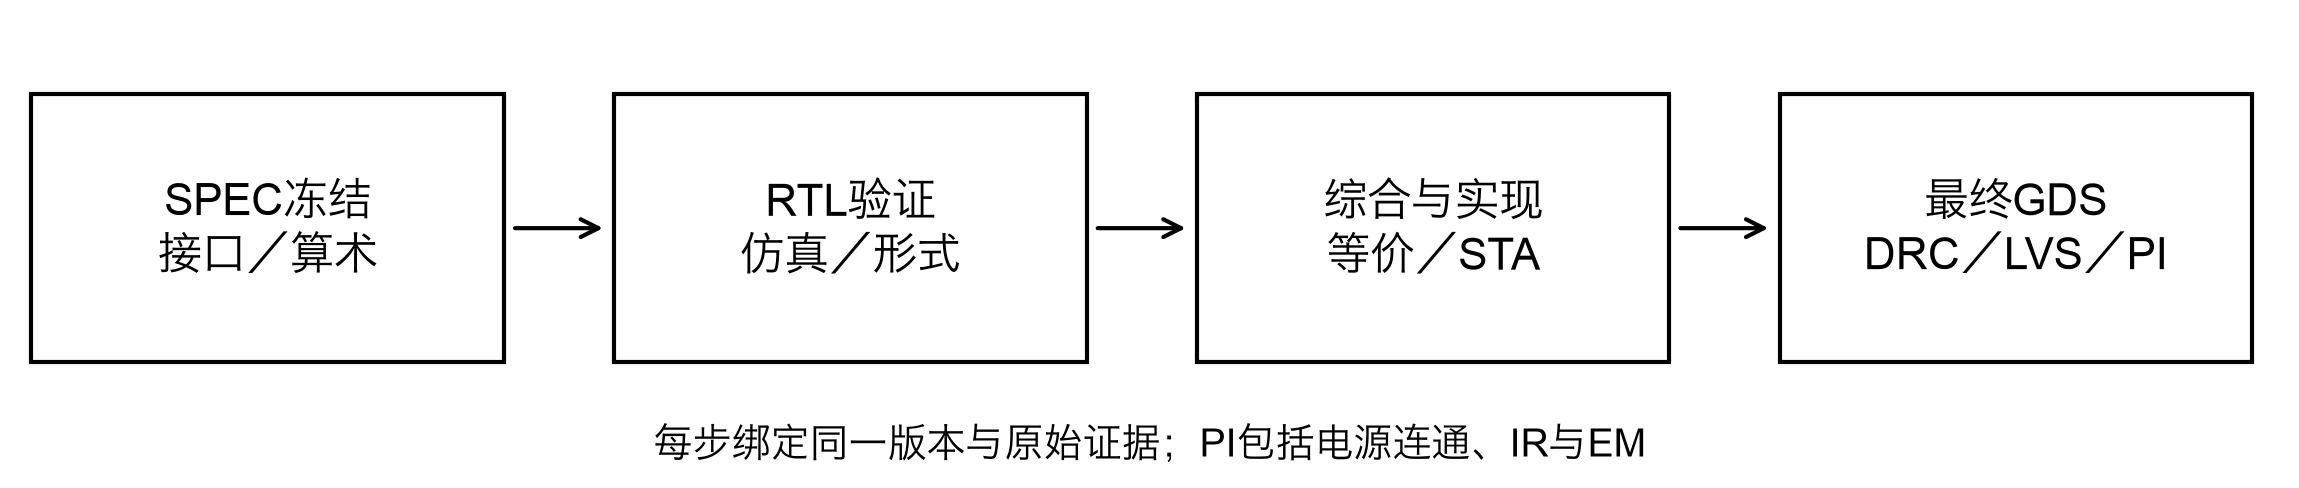
\includegraphics[width=146mm]{figures/signoff_flow.png}
  \caption{拟执行的数字验收链，不表示各环节已经通过}
  \label{fig:拟执行的数字验收链-不表示各环节已经通过}
\end{figure}

\textbf{签核纪律：}逐项标PASS（通过）、FAIL（失败）、BLOCKED（缺前提）、NOT\_RUN（未执行）或PARTIAL（部分完成）。缺工具、规则、角或输入不能标通过；PG／IR／EM、多角STA或等价未完成时，不得宣布完整数字签核。已有66b2e2e的两个控制顶层GDS及TT结果仅作参考，含片上重构的当前整体顶层必须单独交付。180 nm BCD另行实现，不能继承SKY130结果。


\clearpage
\section{接口、首周动作与提交格式}

\begin{table}[H]
\small
  \centering
  \begin{tabularx}{\linewidth}{>{\hsize=0.6\hsize\linewidth=\hsize\raggedright\arraybackslash}X>{\hsize=1.4\hsize\linewidth=\hsize\raggedright\arraybackslash}X}
    \toprule
    模拟组给出／确认 & 学生负责形成的数字合同 \\
    \midrule
    电容连接、可交换组、辅助注入与参考轨 & 主136位／子40位及采样40位的实际映射、位序、极性和名义补偿；工程假设与原文分开 \\
    SADC／ADC2有效时刻、RA增益与窗口、超窗含义 & 9位粗码、12位ADC2、32位样本ID、8个有序片号及六位字的握手／延迟；错误不静默丢弃 \\
    捕获／保持、斩波及AZ确认、CDC／复位条件 & 偶奇极性、AZ代、状态退出、重启与配置更新；每个有源输入都有时序约束 \\
    可选的采集、参考与耦合预算 & 如开展系统敏感性研究则接入样本／等效响应；不作为三项算法行为验收前提，不承担模拟晶体管设计 \\
    \bottomrule
  \end{tabularx}
\end{table}

已有数字时序：八片采集描述符在采集请求受理沿N后N+2发布；重构核在E0受理、E22出结果。16拍一笔是吞吐目标，不是单笔延迟。现有整体合同要求模拟宏在N+15前提交ADC2，必须在接口冻结时与实际孔径、RA时窗核对，不能据数字仿真声称模拟已满足。

\textbf{权重模式合同：}当前无DEM与Fig.21模式分别训练系数，dither关／开在同一模式内共用冻结系数。不能把``同一LMS流程''误读为任意模式通用同一组数值。默认固定模式运行；更换不兼容模式时先暂停、清空并重载匹配系数。负例只说明配置必须匹配，不是DEM关闭本身的性能。

\begin{figure}[H]
  \centering
  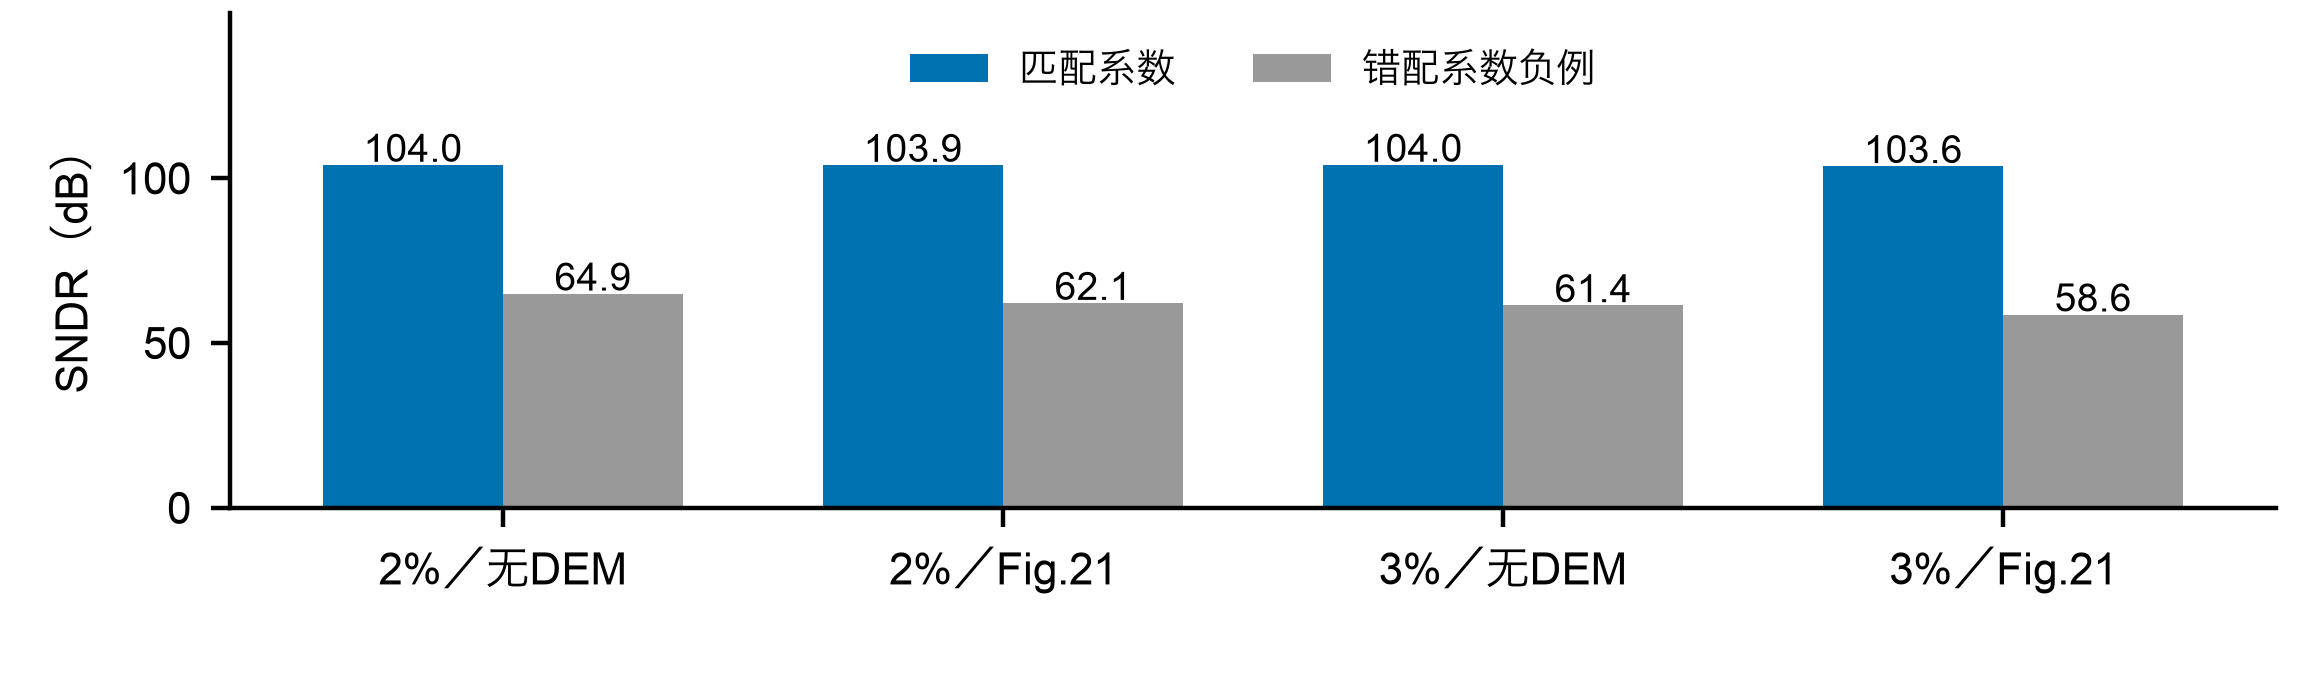
\includegraphics[width=146mm]{figures/coefficient_mode.png}
  \caption{系数组错配负例：正确配置均有约103 dB，错装另一映射模式权重会失效；不是DEM关／开的公平对照}
  \label{fig:系数组错配负例-正确配置均有约103-db-错装另一映射模式权重会失效-不是dem关-开的公平对照}
\end{figure}

直接代码起点：task1的module1\_bridge\_top、task2的dither8\_top、task3的caaz20\_pair，以及task\_reconstruction的sar20\_lms\_recon。复用其模型、TB和检查脚本；具体端口以各自SPEC为准。

首周：固定提交与工具版本，运行现有Python回归，抽查已有数据／图；查看模块一、dither和重构匹配记录，再核对两份整体记录的物料身份，变化部分才定向重放。已有RTL不重复实现，旧收据不重签。只有相关输入或实现改变时，才重新训练并重跑相应实验。

每阶段提交``运行说明＋配置／种子／输入＋原始结果＋效果图＋测试日志''；最终再交``spec／需求对应＋RTL／综合网表＋GDS／SDC／SPEF＋签核报告＋摘要清单''。训练／留出分离，禁止用真实失配作训练答案。LSB20统一为$10/2^{20}$~V，所有图注明码范围、带宽、样本／命中数、LMS状态与适用边界。

项目范围固定：ISSCC的9位前级及18／8架构，三个数字工作包与必要的重构／集成。行为级以电荷／码关系、失配校准、样本噪声及数字对齐为主；复杂动态仅作可选扩展。本期不扩展DSP、CICC后级架构、模拟RA设计或片内LMS训练器。

参考：Bodnar等，ISSCC 2024 9.8，论文1页及Fig.9.8.1／3；US10516408B2（切片转换级）、US10511316B2 Fig.11／20／21（DEM）、US10505561B2 Fig.3／19（dither）；Wang等，VLSI 2025 C32-1 Fig.5／6（CAAZ）。采集前tracking、输入充电辅助及低功耗参考分别另见US10707889B1、US10541702B1、US10826519B1；不因引用而声称已实现。原件和代码入口统一见仓库README与references索引。

原图与短句均按用户要求节选自其提供的原件，版权归原权利人；软件许可不覆盖原图。图页、文字页、裁剪与SHA256分别记录在source\_figures.json，不把原图中的电路画成已实现状态。

更新记录：2026-11-08，以aea7d1f工作树及归档记录编制；只新增接手文档、计划图及排版源，不修改算法、RTL或实验数值。任务书定义未来验收，未新增任何数字签核通过结论。


\clearpage
\section{技术说明：交织、量化器与残差DAC怎样分工}

\begin{figure}[H]
  \centering
  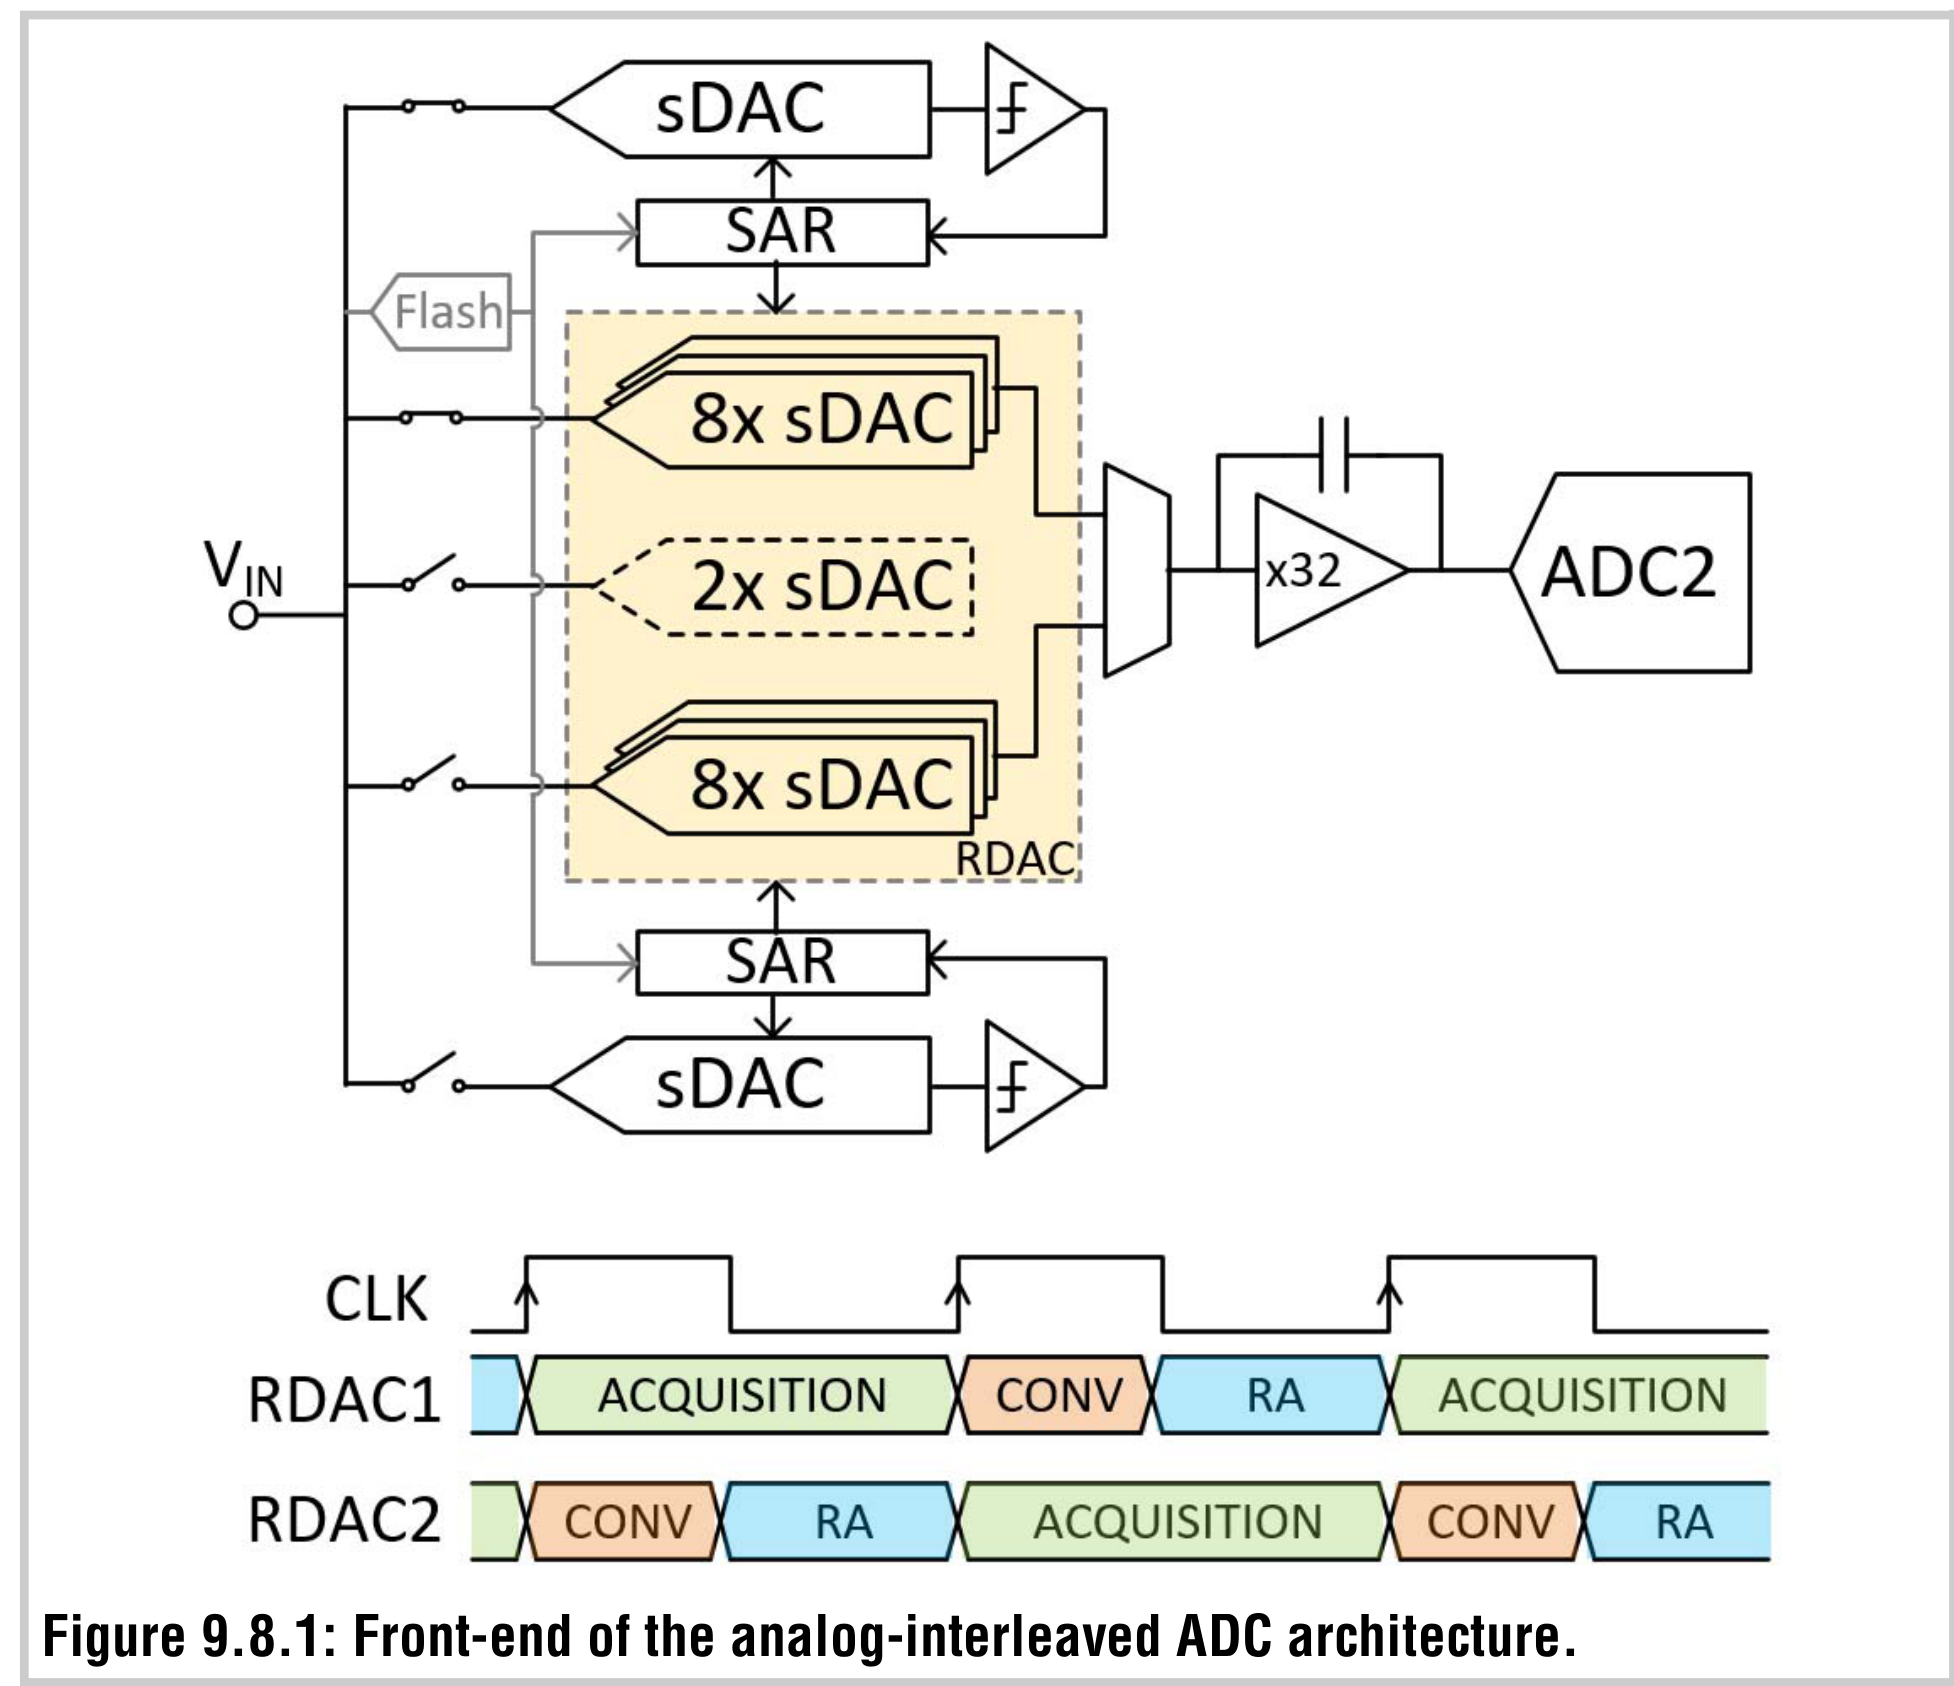
\includegraphics[width=132mm]{figures/source_isscc_architecture.png}
  \caption{ISSCC 2024原论文Fig.9.8.1，PDF第2页、印刷183页：模拟交织前级及采集／转换／RA时序；©~IEEE}
  \label{fig:isscc-2024原论文fig-9-8-1-pdf第2页-印刷183页-模拟交织前级及采集-转换-ra时序-ieee}
\end{figure}

\textbf{沿原图读信号：}VIN同时服务小量化器和大残差DAC。量化器先得到粗码，RDAC按结果建立残差，RA再把残差送ADC2。RDAC的18个切片不是18路独立输出ADC：每笔8片共同采集，另8片共同形成上一笔残差，2片留作重排资源。

\textbf{为什么要交织：}当前8片转换时，下一组8片可以跟踪输入；输入采集延长至一个原始周期。项目10 MS/s时T=100 ns。固定的采集／转换两组容易把失配变成周期杂散，随机改变物理组可打散这些杂散，但也可能提高宽带误差。时偏和采样带宽不匹配仍需控制，不能只靠随机调度解决。

\textbf{时序关系必须一起成立：}转换组来自上一采集组；采样孔径之前控制字已稳定；本笔ADC2孔径与下一输入孔径对齐。16个数字tick是工程分配，不是原文完整时序。原图的RA倍率和$\pm$3 V、40 MS/s条件不能直接搬到本项目的$\pm$5 V、10 MS/s。

\textbf{复现要求：}学生复用现有调度器，交每片角色与样本ID随时间图，验证无重复占用、stall不推进、同笔配置保持。模拟组给孔径、释放与RA时窗；数字侧冻结受理沿与延迟。资源组随机选择与片内单元DEM分别统计，不能混为同一个开关。


\clearpage
\section{技术说明：Fig.11电容网络与桥接权重}

\begin{figure}[H]
  \centering
  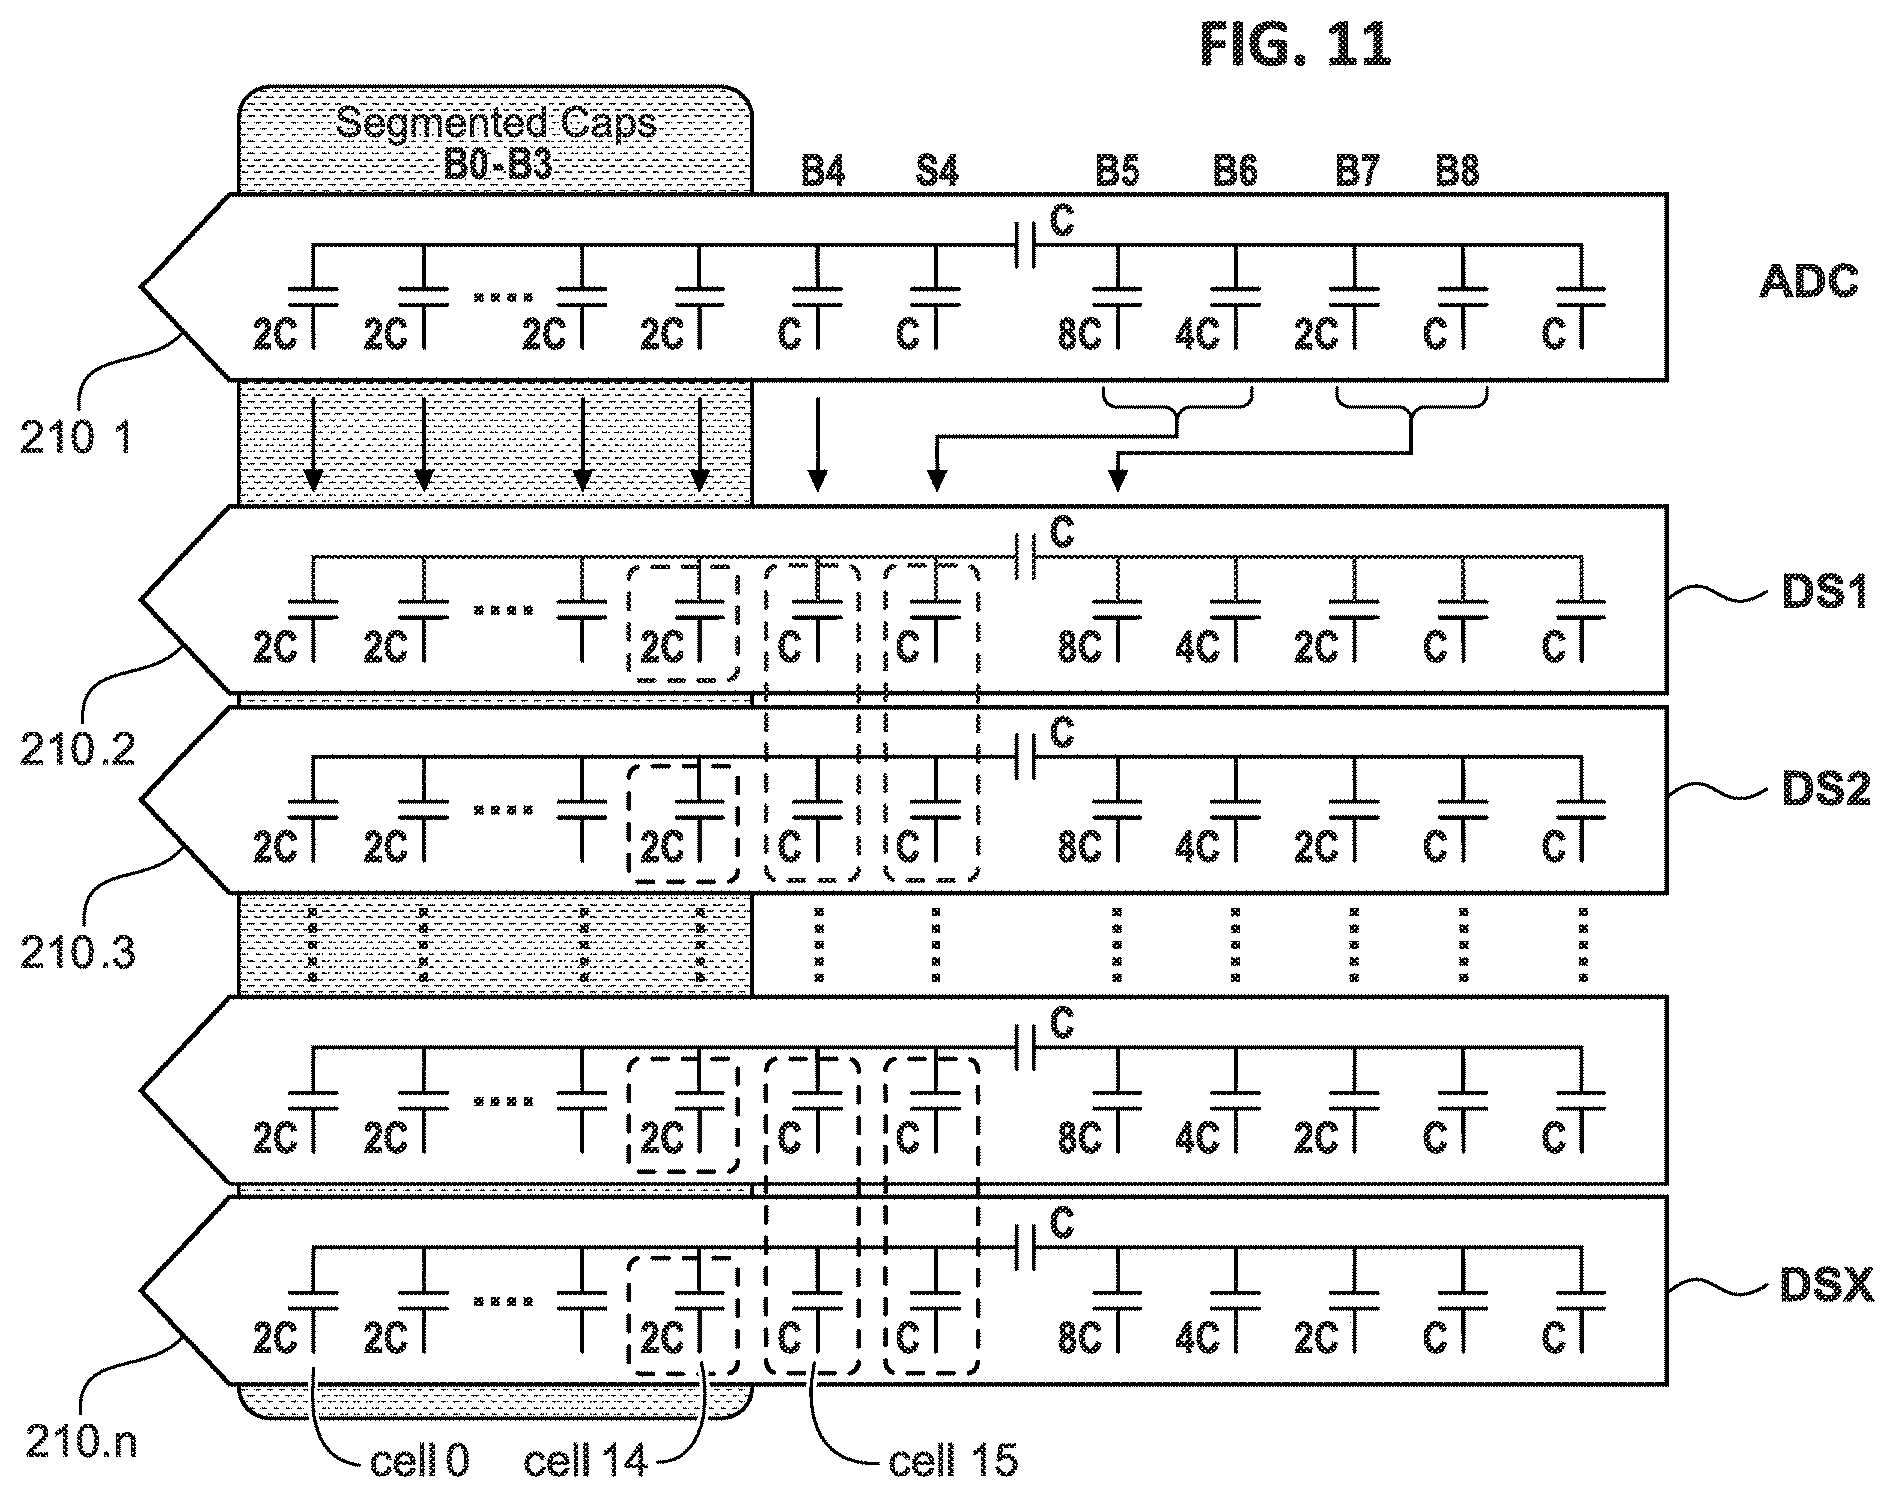
\includegraphics[width=140mm]{figures/source_dem_fig11.png}
  \caption{US10511316B2原图Fig.11，PDF第12页；横放原稿已转正，节点和器件保持原样}
  \label{fig:us10511316b2原图fig-11-pdf第12页-横放原稿已转正-节点和器件保持原样}
\end{figure}

\textbf{结构：}B0～B3由分段的2C单元表达，主侧还有B4与S4两个1C；桥接电容把主节点和B5～B8所在子阵列相连。S4不是看到图就能固定当dummy的无关电容：其可切换用途和底板轨必须与模拟组冻结。

以下为静态线性网络分析，不是论文给出的模型公式。定义主／子总电容为C\_M、C\_S，桥接为C\_B；节点v\_M、v\_S相对同一参考，右端q\_M、q\_S为对应电荷激励：

\begin{equation}
(C_M+C_B)v_M-C_Bv_S=q_M,\qquad -C_Bv_M+(C_S+C_B)v_S=q_S.
\end{equation}

消去子节点后：

\begin{equation}
\beta=\frac{C_B}{C_S+C_B},\qquad v_M=\frac{q_M+\beta q_S}{C_M+\beta C_S}.
\end{equation}

所以子电容的作用不能只按名义二进制数相加，桥接与寄生会同时影响权重和增益。Fig.11直接支持C\_B=C及子阵列总16C的名义值；β=1/17还依赖零寄生及连接前提，是推导值而非原文承诺的工艺参数。模型使用输入折算电荷域，足以验证静态权重和数字补偿；v\_M与ADC2实际电压的硬件映射另记。

\textbf{复现要求：}逐单元登记物理连接、采样节点、参考轨、可交换组和dummy状态；用独立两节点求解验证名义与固定失配网络。不能把跨桥的位直接搬到主侧并假设电荷不变，不能用代码当前的1 fF归一单位估计真实kT/C、面积或参考电流。


\clearpage
\section{技术说明：Fig.20／21怎样实现两级DEM}

\begin{figure}[H]
  \centering
  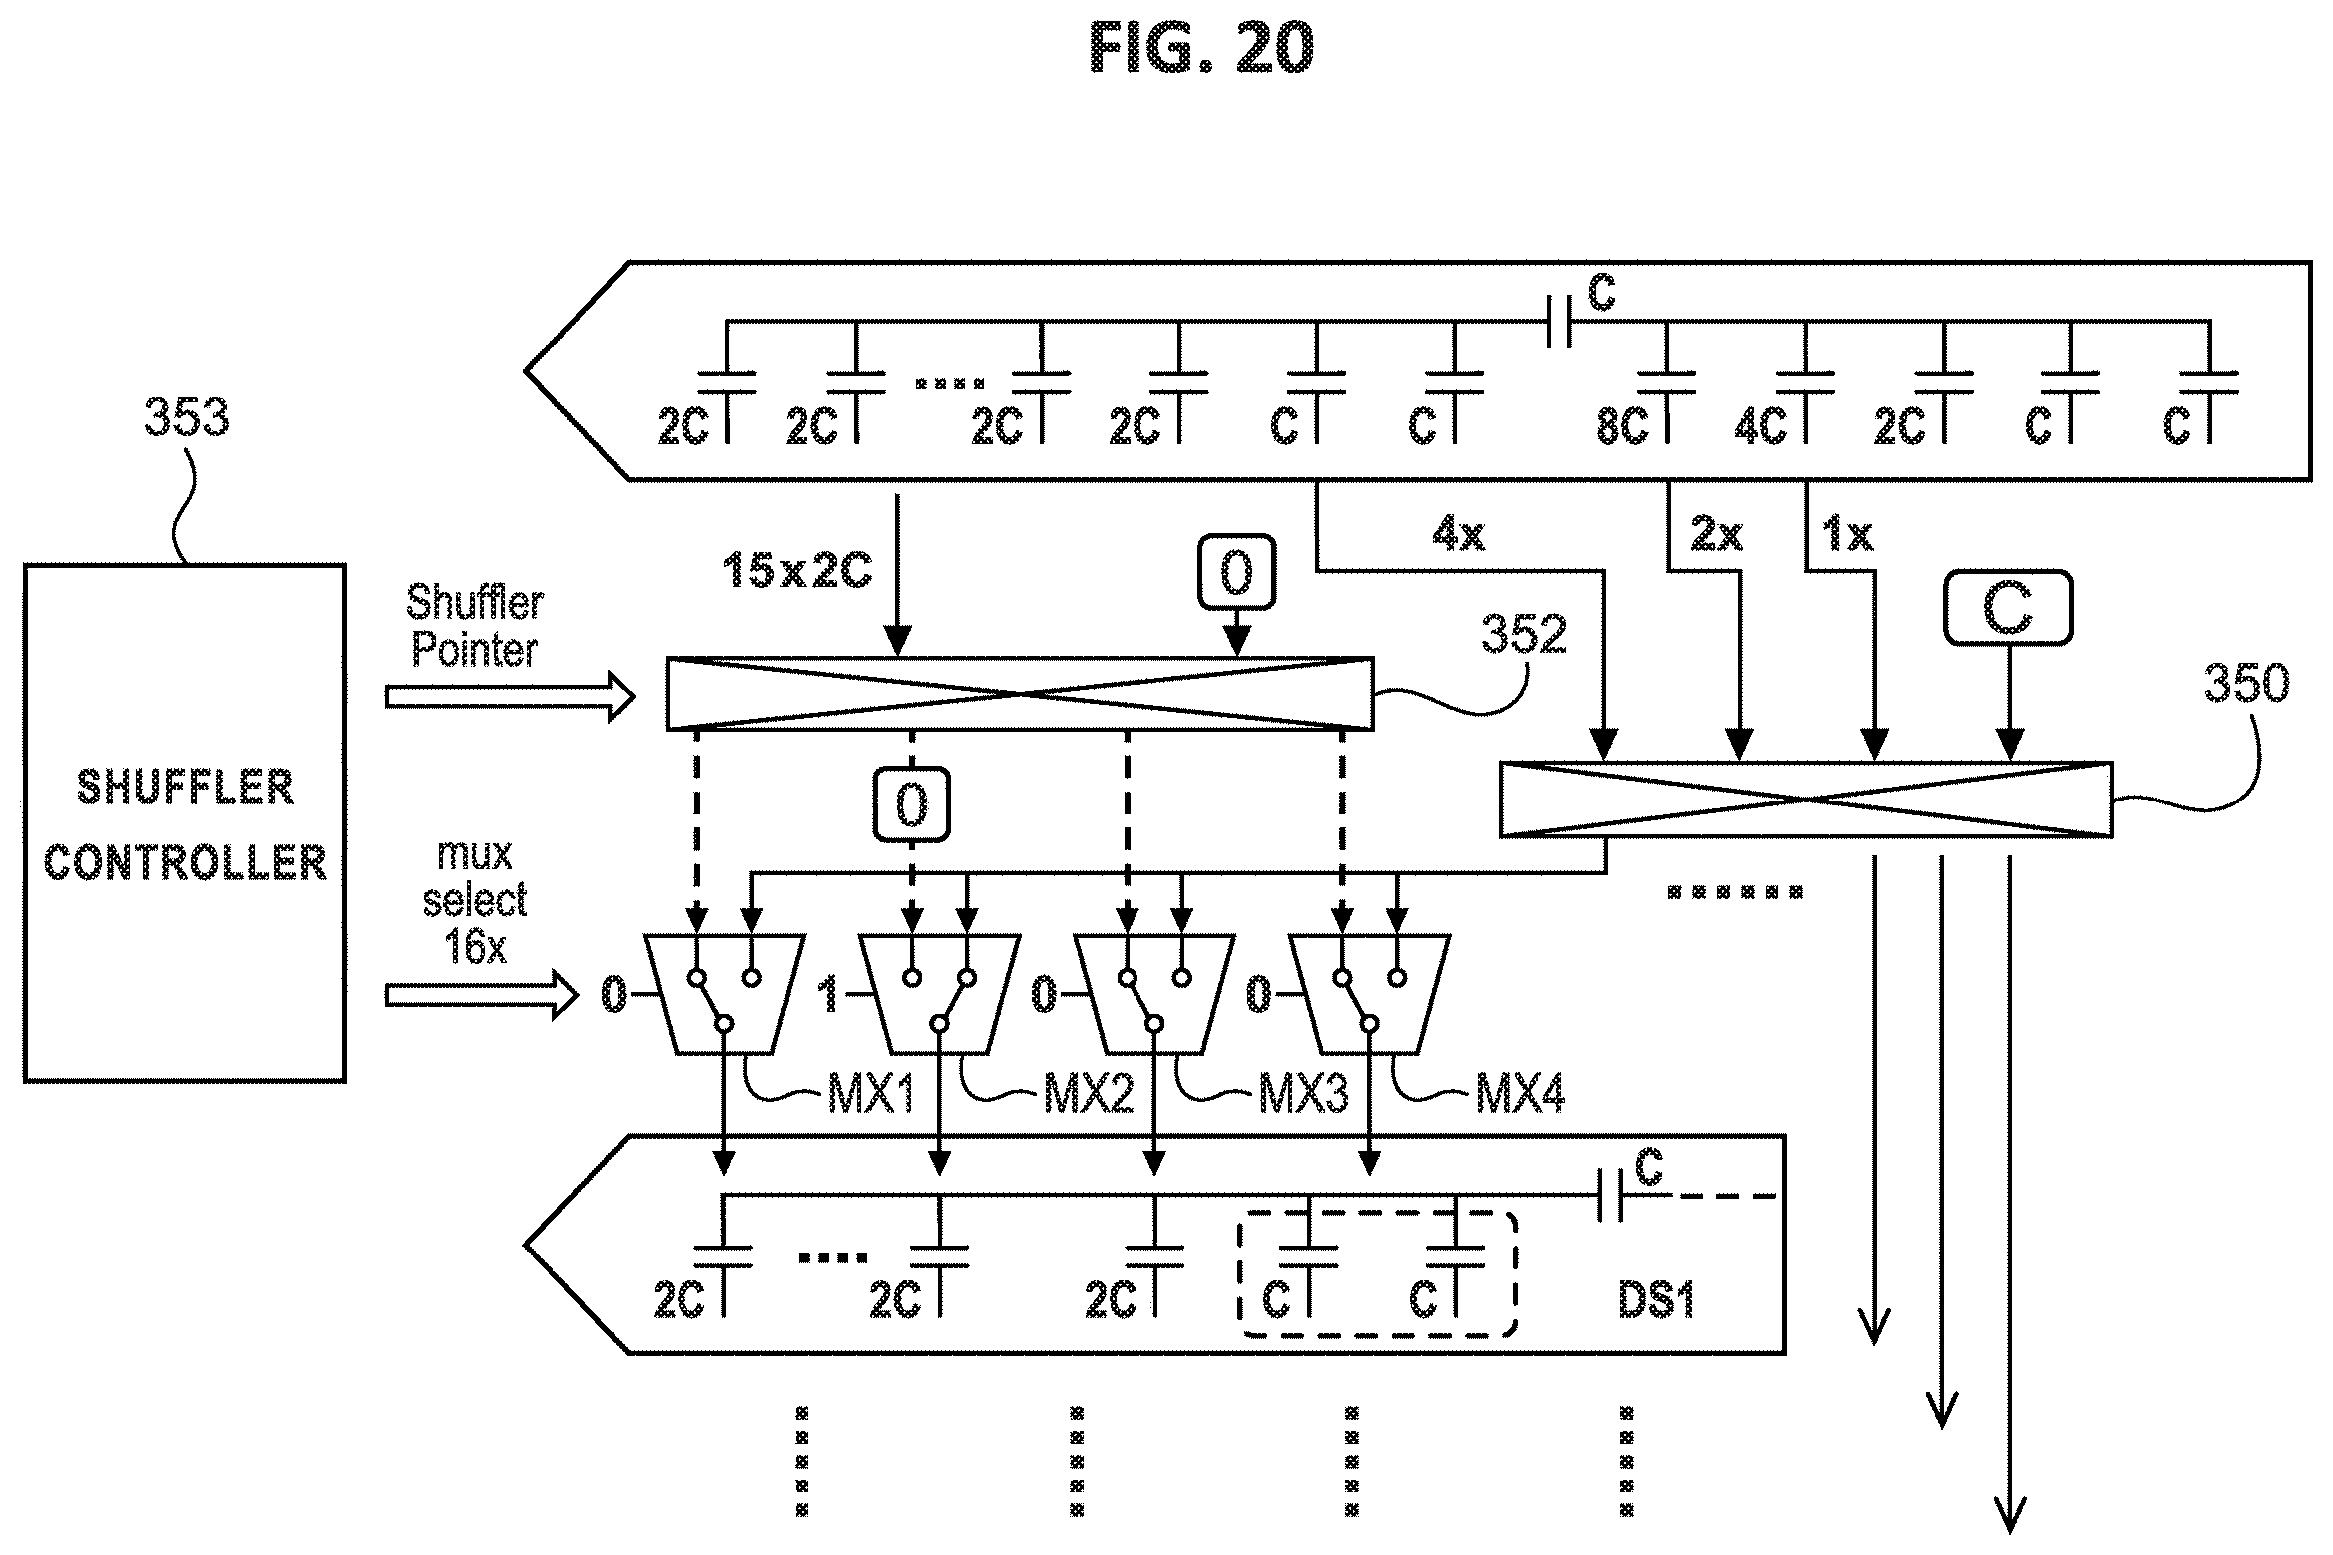
\includegraphics[width=118mm]{figures/source_dem_fig20.png}
  \caption{US10511316B2原图Fig.20，PDF第20页：352、350、MUX与控制器353；原稿转正}
  \label{fig:us10511316b2原图fig-20-pdf第20页-352-350-mux与控制器353-原稿转正}
\end{figure}

\begin{figure}[H]
  \centering
  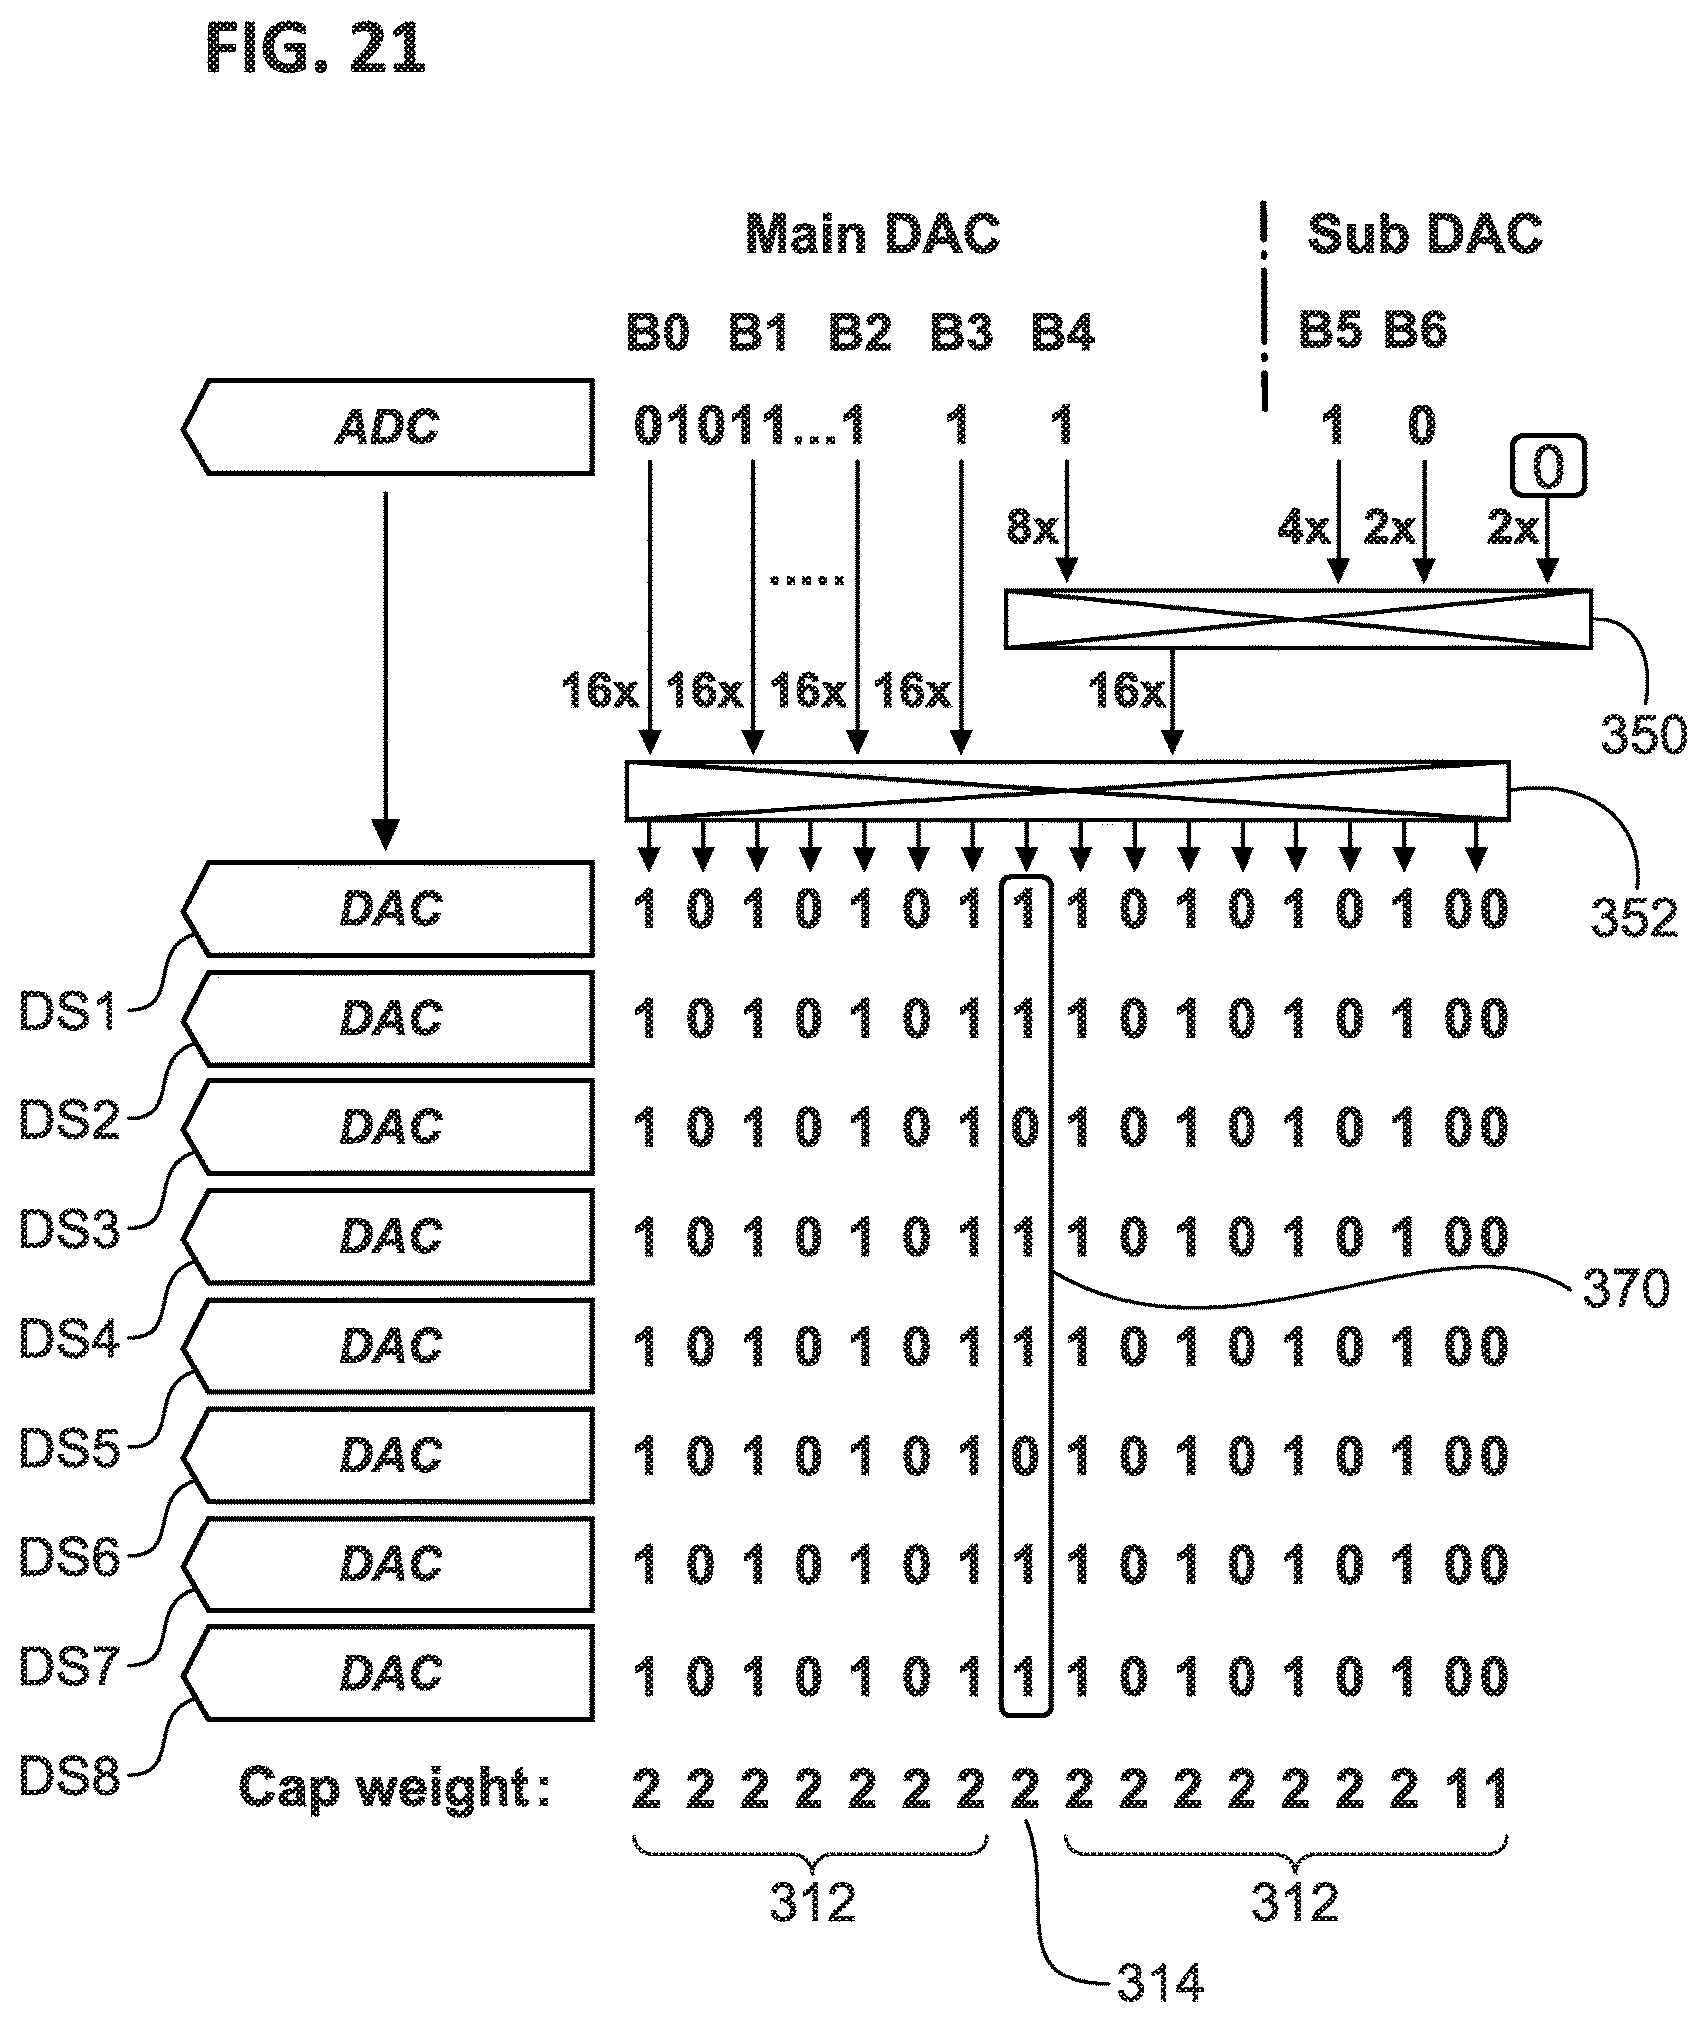
\includegraphics[width=80mm]{figures/source_dem_fig21.png}
  \caption{同专利原图Fig.21，PDF第21页：保留列370在片间分配；与Fig.20配合阅读}
  \label{fig:同专利原图fig-21-pdf第21页-保留列370在片间分配-与fig-20配合阅读}
\end{figure}

352把预留输入0和主段一元字重排到物理列；353据该位置控制MUX，选定列改由350驱动，其余列沿352。350负责相应列在八片中的选择。因此必须同时核对``保留了哪一列''及``哪些片用了它''，不能只做一层轮转。

\textbf{原句：}同专利PDF第42页、印刷21栏，Fig.21说明末段：

\begin{quote}
``This shuffling scheme further reduces the impact of size errors between the cells and gives rise to further improvements in INL errors.''
\end{quote}

原文说改善单元尺寸误差与INL，没有给本工程2\%／3\%池的收益。其对应的控制规则、工程跨段补偿和效果证据继续在下一节推导。


\clearpage
\section{技术说明：DEM为何有收益，为什么仍需LMS}

对某一固定制造池，设单元误差为δC\_i，选择状态为s，输入码为c。将已确认网络的有效灵敏度记为a\_i(c,s)，则一阶误差可写为：

\begin{equation}
e(c,s)\simeq\sum_i a_i(c,s)\delta C_i.
\end{equation}

固定映射使误差随码重复，形成INL结构与杂散。DEM改变状态s，使一部分误差从确定性失真转为波动；但条件均值E[e|c]不一定为0。只看到杂散下降，不能据此宣称SNDR、单次精度或使用均匀性同时达标。固定池必须贯穿全部对照，不能每笔重新抽电容。

\textbf{跨段不能遗漏补偿：}令H为B0～B3的4位值、m=4B4+2B5+B6。保留列方案的主侧名义量为16H+2m（单位C）。在本工程β=1/17、旧码表和对称参考约定下，迁移B5／B6相对旧网络多出的选择电容为：

\begin{equation}
\delta C=\frac{4B5+2B6}{17}C.
\end{equation}

输入折算补偿最大约10 V$\times$6/(17$\times$256)=13.79 mV。这个数来自工程网络，不是专利规格。沿旧码表重构时补一次；若直接按迁移后的真实位权重构，不能再重复加。数字补偿不能挽救已经超出RA／ADC2窗口的样本。

\textbf{LMS做另一件事：}它从可用观测估计固定权重，减小δC\_i的重构影响。训练后冻结，再用独立留出评价。论文披露外部系数与片上位权修正，具体LMS、Q28和更新接口是工程选择。动态建立误差并不会因为用了静态LMS就自动消失。

\textbf{逻辑相位不能代替物理统计：}当前15态映射八起点不均，但实际18片组也在变化。固定码专项100,000笔中，各物理片选中5432～5668次；当前／独立均匀起点的条件单元使用偏差RMS约5.044\%／5.034\%。据此不能判为DEM行为缺陷。应结合物理mask、输入条件和INL／频谱裁定，避免把逻辑索引计数当作电容失配效果。

\begin{table}[H]
\small
  \centering
  \begin{tabularx}{\linewidth}{>{\hsize=0.6\hsize\linewidth=\hsize\raggedright\arraybackslash}X>{\hsize=1.4\hsize\linewidth=\hsize\raggedright\arraybackslash}X}
    \toprule
    复现对象 & 必须看到的证据 \\
    \midrule
    机制正确 & 全码／合法相位下的独立电荷关系，保留列与物理mask对齐，补偿漏加／双加负例 \\
    统计效果 & 同池DEM$\times$LMS四组INL／DNL、频谱、训练收敛；同时报告均值误差和波动 \\
    原文对齐 & 未实现的开关或可交换关系单列；不能把当前受限候选写成完整原型3D DEM \\
    \bottomrule
  \end{tabularx}
\end{table}


\clearpage
\section{技术说明：减性dither为什么能平滑码边界}

\begin{figure}[H]
  \centering
  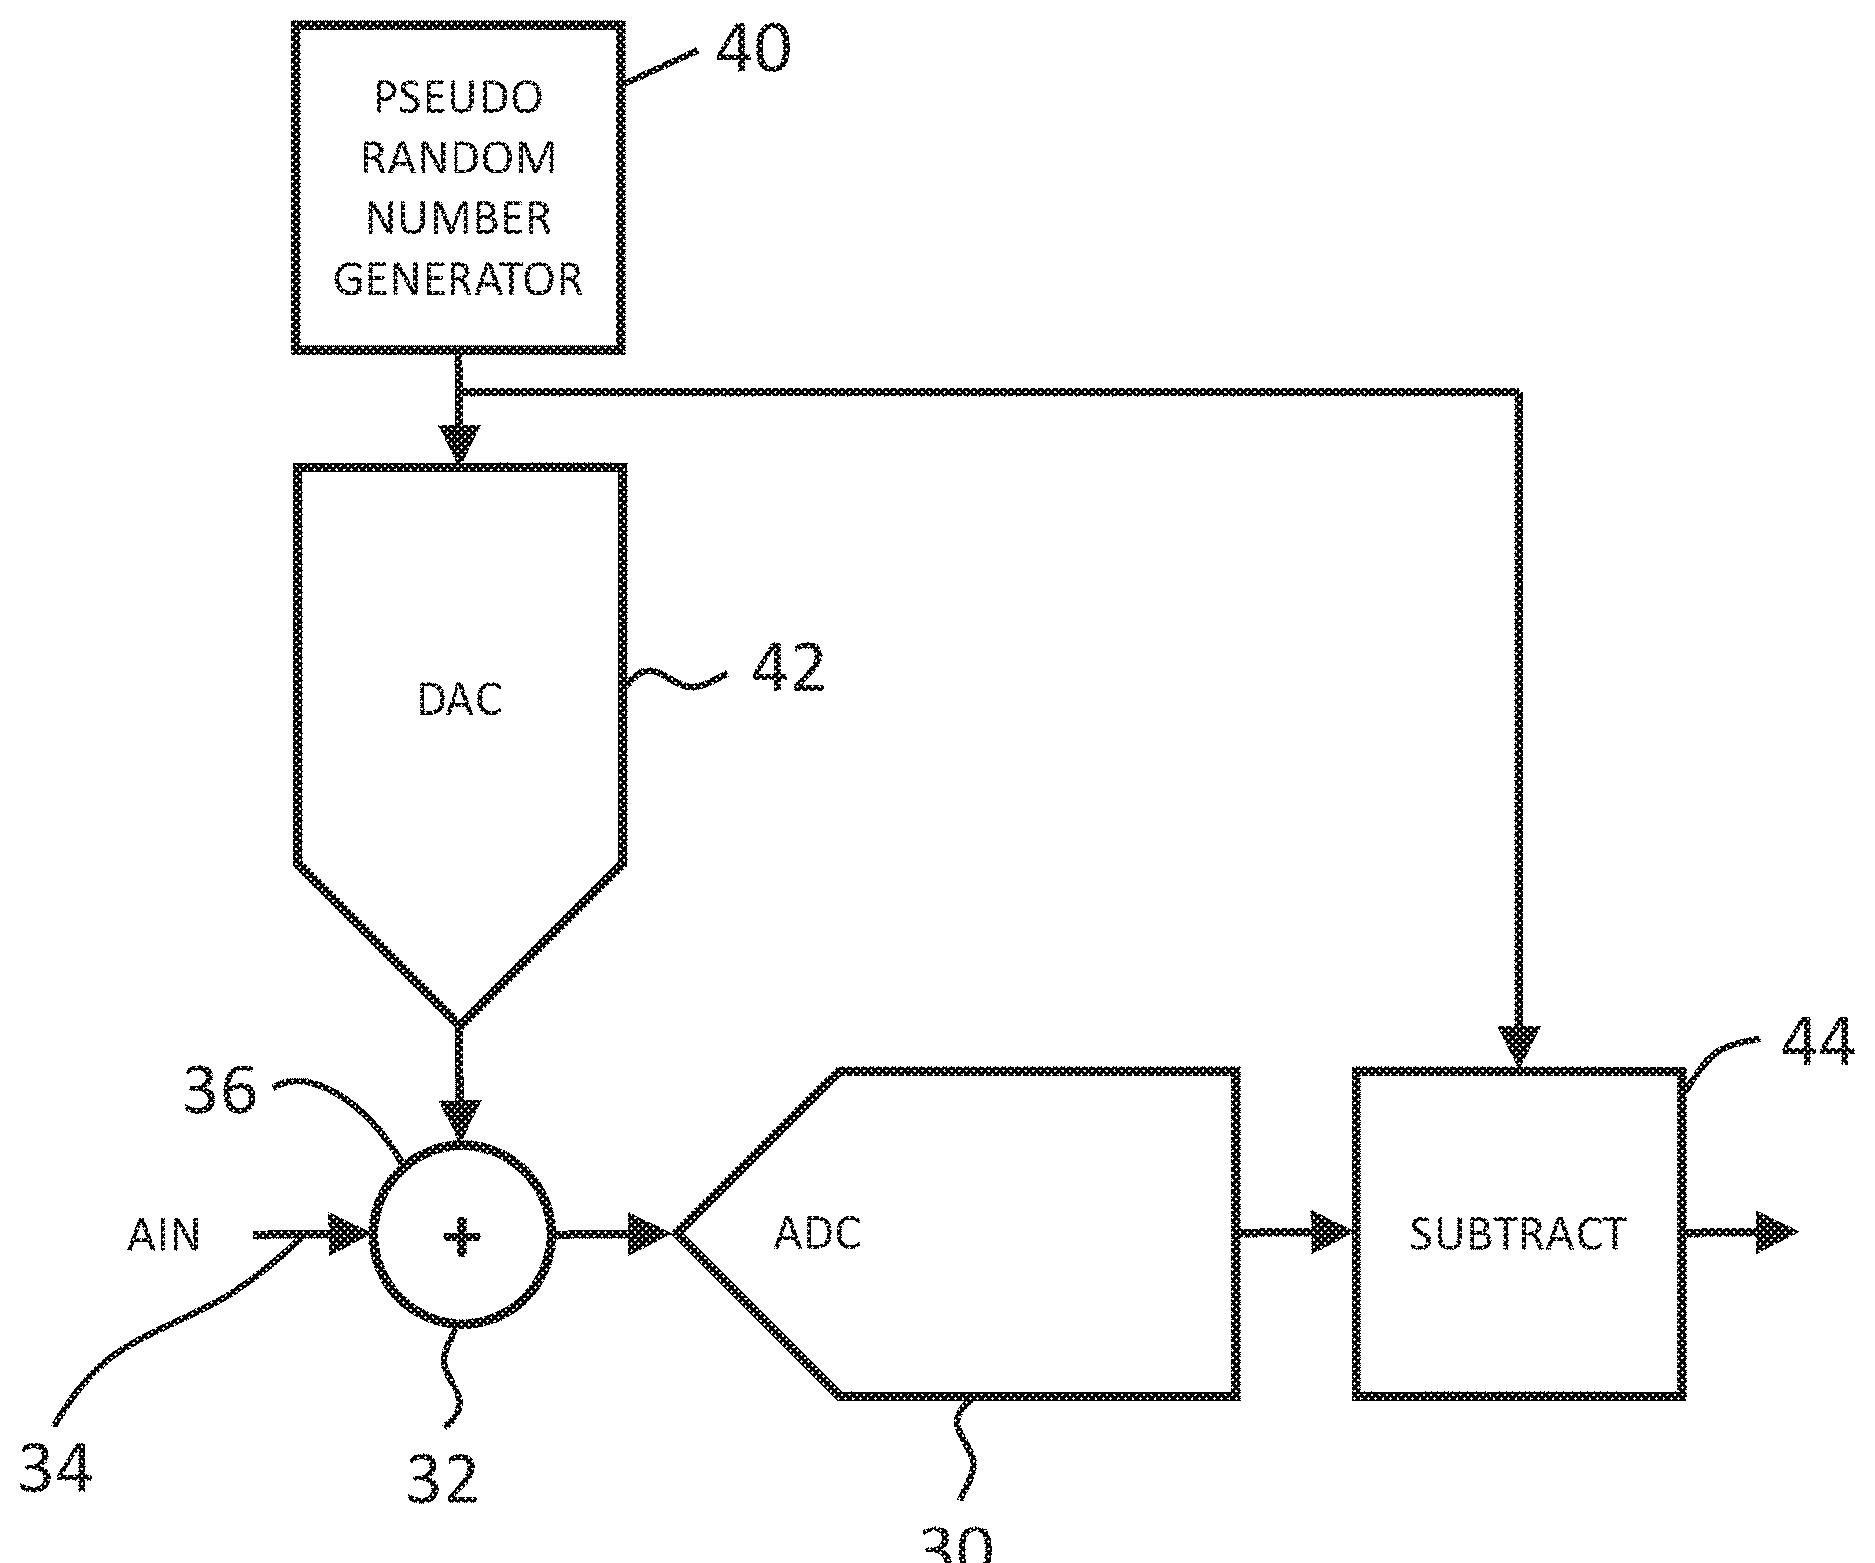
\includegraphics[width=112mm]{figures/source_dither_fig3.png}
  \caption{US10505561B2原图Fig.3，PDF第5页：同一伪随机字驱动模拟注入与数字减法}
  \label{fig:us10505561b2原图fig-3-pdf第5页-同一伪随机字驱动模拟注入与数字减法}
\end{figure}

\textbf{原句：}该专利PDF第26页、印刷第5栏，Fig.3说明：

\begin{quote}
``The dither signal is formed in the digital domain by a pseudo-random number generator 40.''
\end{quote}

随机字d已知，模拟侧转换x+d，数字端去除同一d，得到z=Q(x+d)--d。固定x会落到不同码边界，评价的是E[Q(x+d)--d]。非均匀码宽造成的局部误差因此可能被平滑；这不等于每一笔误差消失，也不保证所有输入、频率和失配下SNDR提高。

原图最关键的不是``加一份噪声''，而是两条支路必须描述同一笔注入。幅度、符号、路径、延迟有误，数字去除就会留下与字相关的误差；ADC过载后再减d也不能恢复丢失的信息。

\textbf{复现要求：}先用理想量化器验证符号和延迟，再接含固定电容失配的电荷网络。记录实际注入权重而不只记录PRNG字；保留dither关／开、无LMS／冻结LMS对照。DEM与dither随机状态独立，并明确stall、禁用、重置和种子重载时的行为。


\clearpage
\section{技术说明：Fig.19六位字如何拆分和落到切片}

\begin{figure}[H]
  \centering
  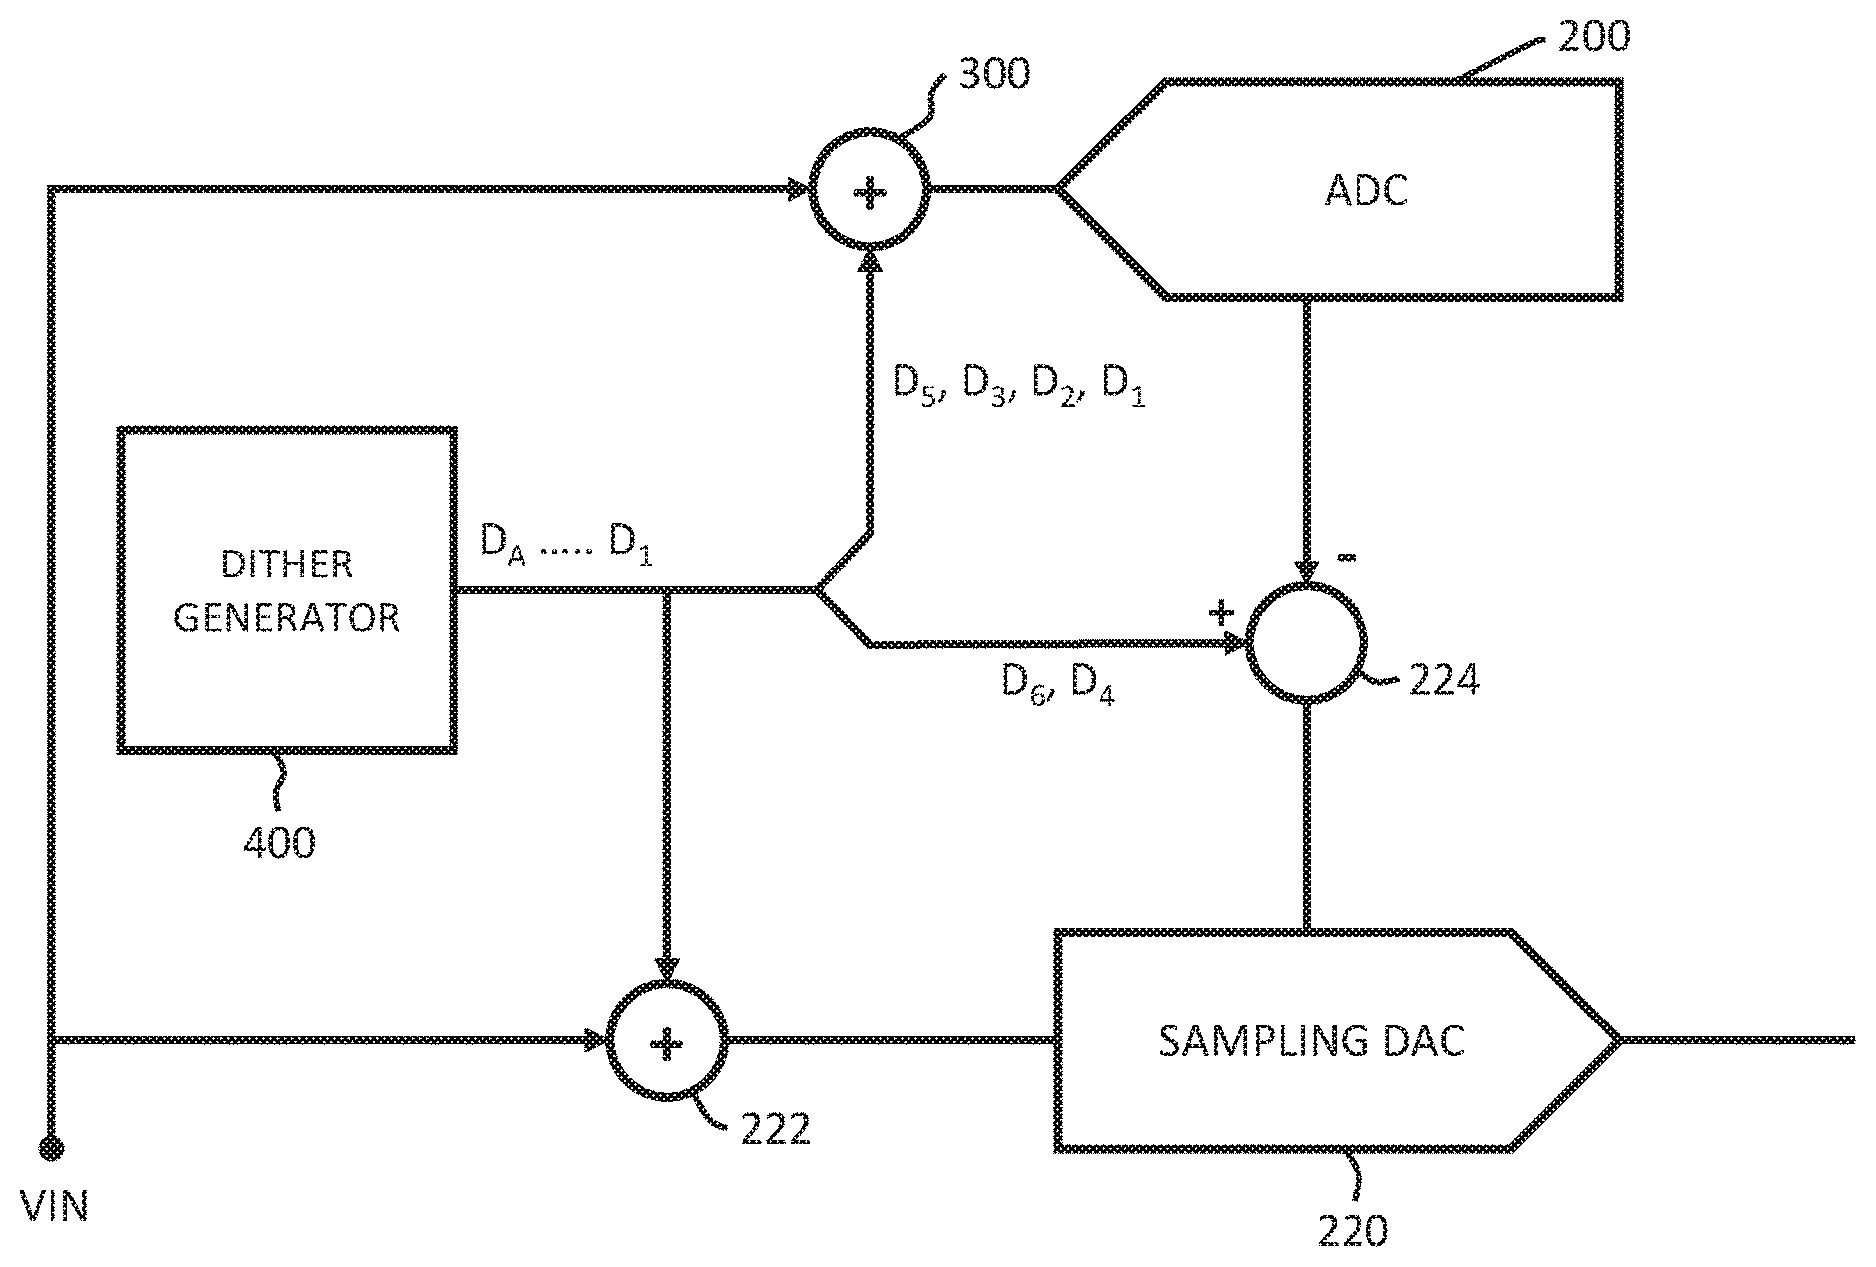
\includegraphics[width=132mm]{figures/source_dither_fig19.png}
  \caption{US10505561B2原图Fig.19，PDF第22页：SADC子字、RDAC全字与224粗码处理}
  \label{fig:us10505561b2原图fig-19-pdf第22页-sadc子字-rdac全字与224粗码处理}
\end{figure}

原文七片示例以一个前级档为单位，令F=4D3+2D2+D1、U=4D6+D4，则L=2D5+F/7、T=L+U。SADC只用D5／D3／D2／D1，RDAC使用全字；PDF第33页、印刷第19--20栏正文规定扣除U，再设置RDAC。图中224符号的方向必须结合码约定和电荷极性阅读。

\textbf{本工程八片约定单独验证：}令m=D[2:0]、U=4D[5]+D[3]、I=U+2D[4]。前m个有序槽取I+1，其余取I，因此名义平均档位为I+m/8；L8=16D[4]+m，T8=8U+16D[4]+m。使用哪几个实际电容由物理mask和权重决定，不由平均值自动保证。

\textbf{可手算的工程例：}D6=1、D5=D4=0、m=3时，U=4、L=3Δ/8、T=35Δ/8；3个槽取5档，5个槽取4档。粗码c=100时k=96；若c=2则必须拒绝下溢，不能回绕。Δ=10/544 V来自当前工程网络，不是原文工艺参数。

\textbf{复现要求：}枚举64个字、全部有序槽和合法相位，检查实际电荷、粗码和去扰。原文/7与工程/8分别记账；确认辅助参考误差是否与转换权重共享。必须把字、逐片电荷、残差及重构连起来核对；当前该行为路径已有独立节点验证，不要求学生先做开关瞬态。


\clearpage
\section{技术说明：分路注入、残差与数字去扰如何闭合}

\begin{figure}[H]
  \centering
  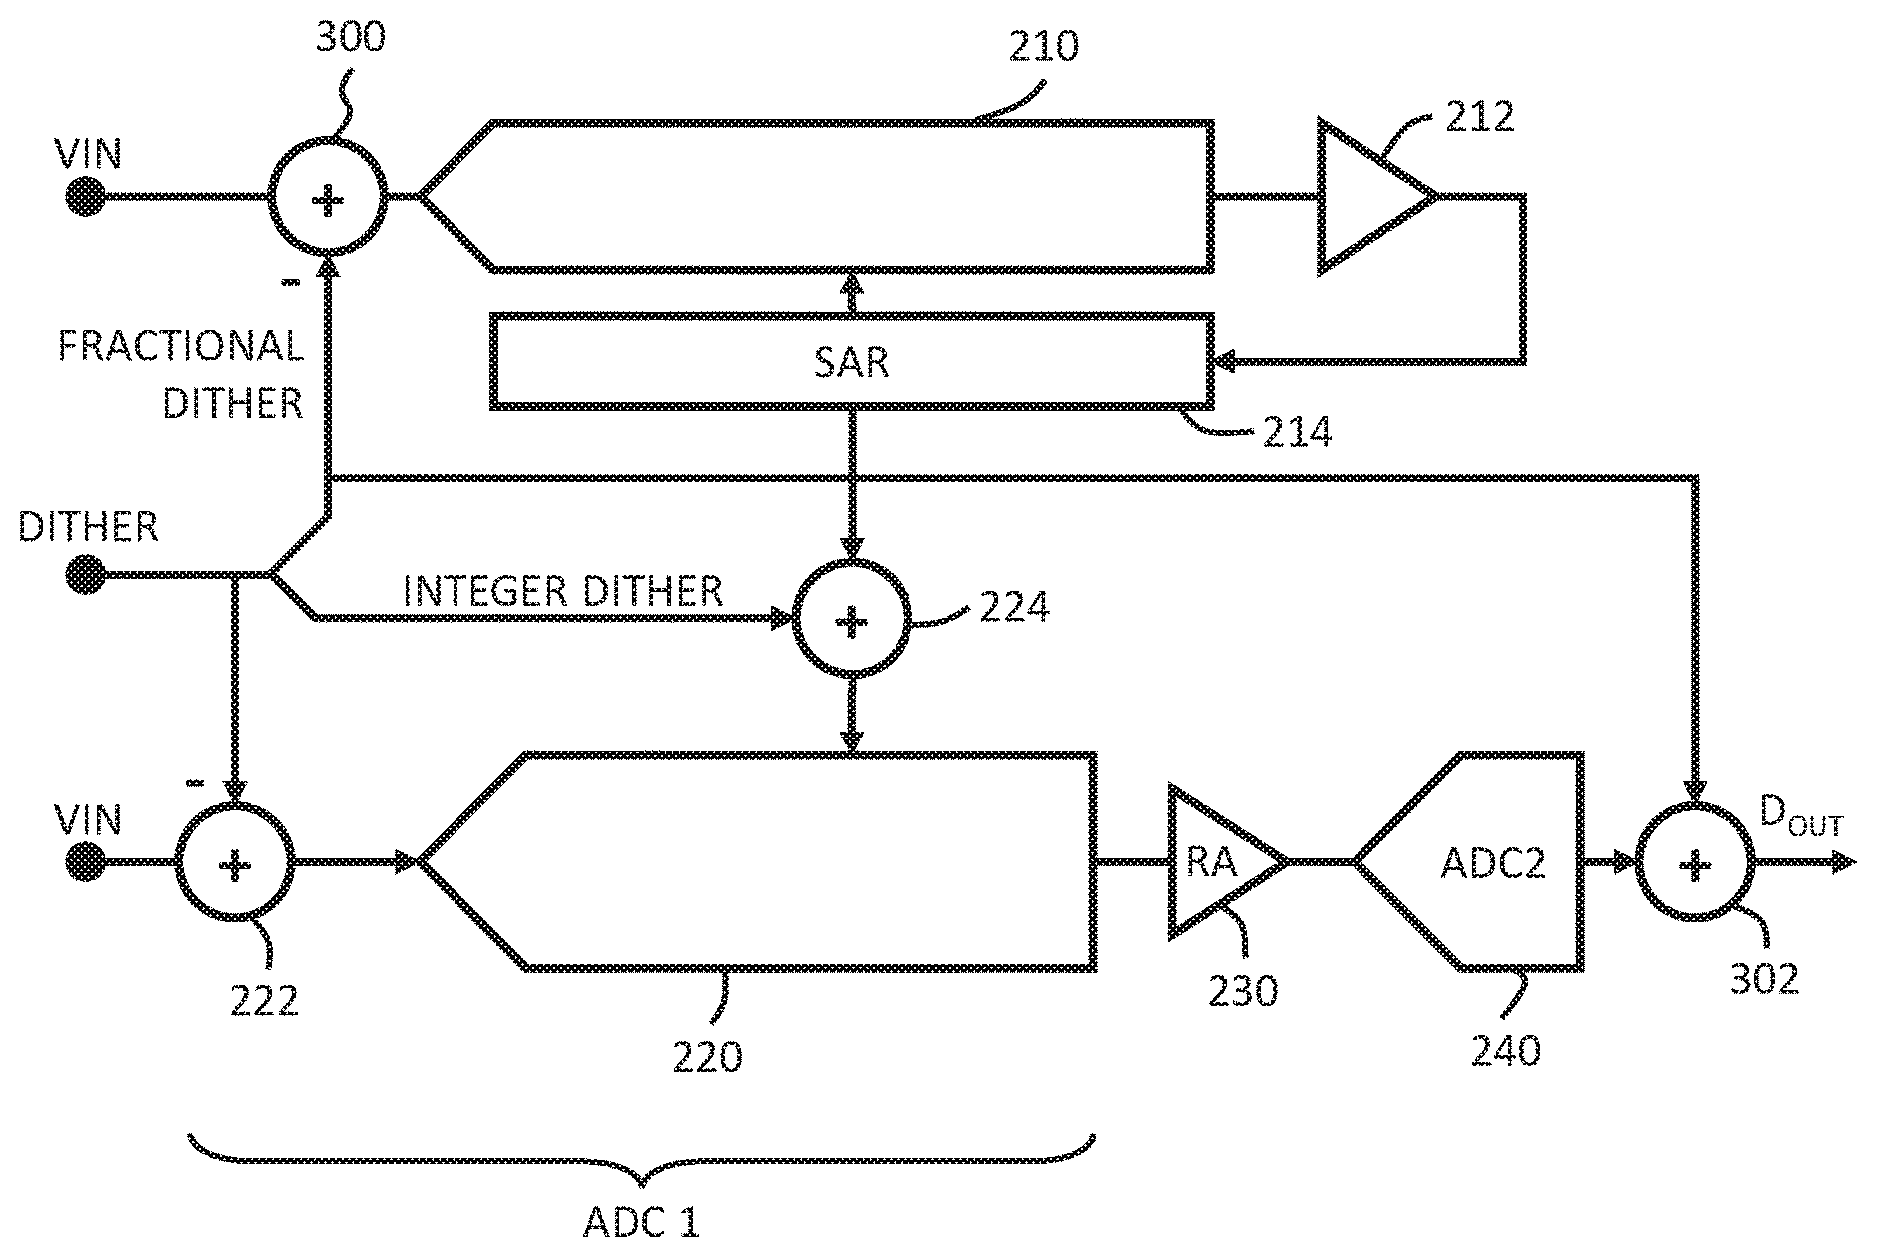
\includegraphics[width=120mm]{figures/source_dither_fig5.png}
  \caption{US10505561B2原图Fig.5，PDF第7页：分路注入、RA／ADC2及输出302补偿}
  \label{fig:us10505561b2原图fig-5-pdf第7页-分路注入-ra-adc2及输出302补偿}
\end{figure}

\begin{figure}[H]
  \centering
  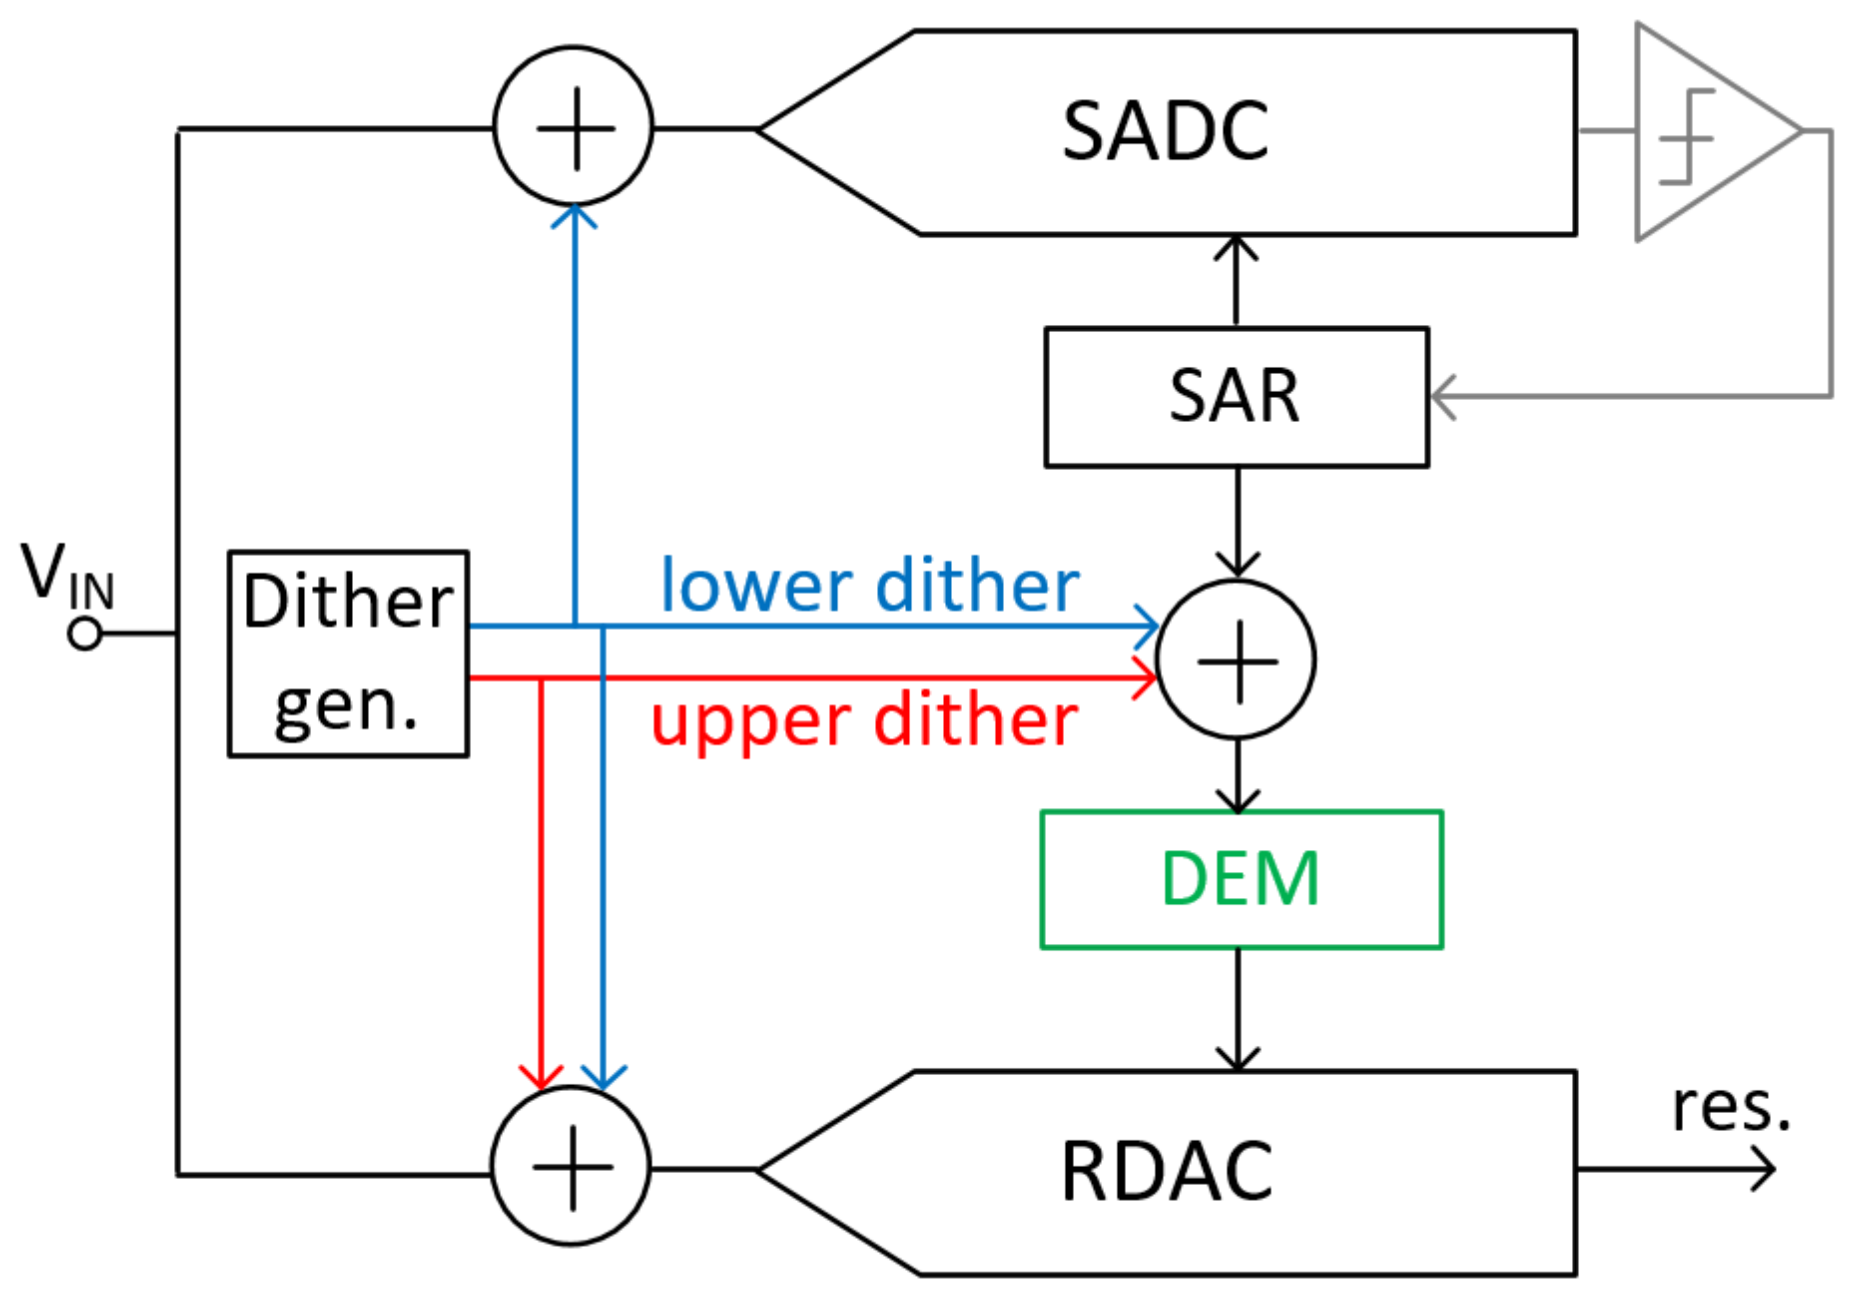
\includegraphics[width=100mm]{figures/source_dither_slide17.png}
  \caption{ISSCC 2024讲稿第17页右侧原图：lower／upper及DEM前码处理；©~IEEE}
  \label{fig:isscc-2024讲稿第17页右侧原图-lower-upper及dem前码处理-ieee}
\end{figure}

ISSCC论文PDF第1页、印刷182页原句：

\begin{quote}
``Dither is used to complement the DEM linearization of the DAC.''
\end{quote}

在当前工程的负注入、输入折算电荷约定下：c=Q(x--L)、k=c--U、r=g(x+5)--VD(k)--T，重构为(r+VD(k)+T)/g--5。T由同笔实际采样mask参与位权重构；不能再按名义T扣／加一遍。conv\_sub+sample\_sub可为2，这是同权重被两项使用，不是非法二进制位。~Fig.3的加性示意与这里的负注入属于不同符号约定，模拟与数字必须整体一致。受控负电荷源是合法行为模型；需核对完整电荷／码路径，而非要求先实现器件开关。实际电路接法由模拟组另行验证。

\textbf{复现要求：}对SADC、RDAC、残差、ADC2和最终码分别画余量；不能只看最终码未clip。全部字下共同名义下限--4.855239 V是尚需处理的目标差距。实际轨、RA增益、采样参考与转换参考不一致时，须更新物理模型及训练合同，而不是调整符号去迎合结果。


\clearpage
\section{技术说明：北大Fig.5把斩波放在哪，数字做什么}

\begin{figure}[H]
  \centering
  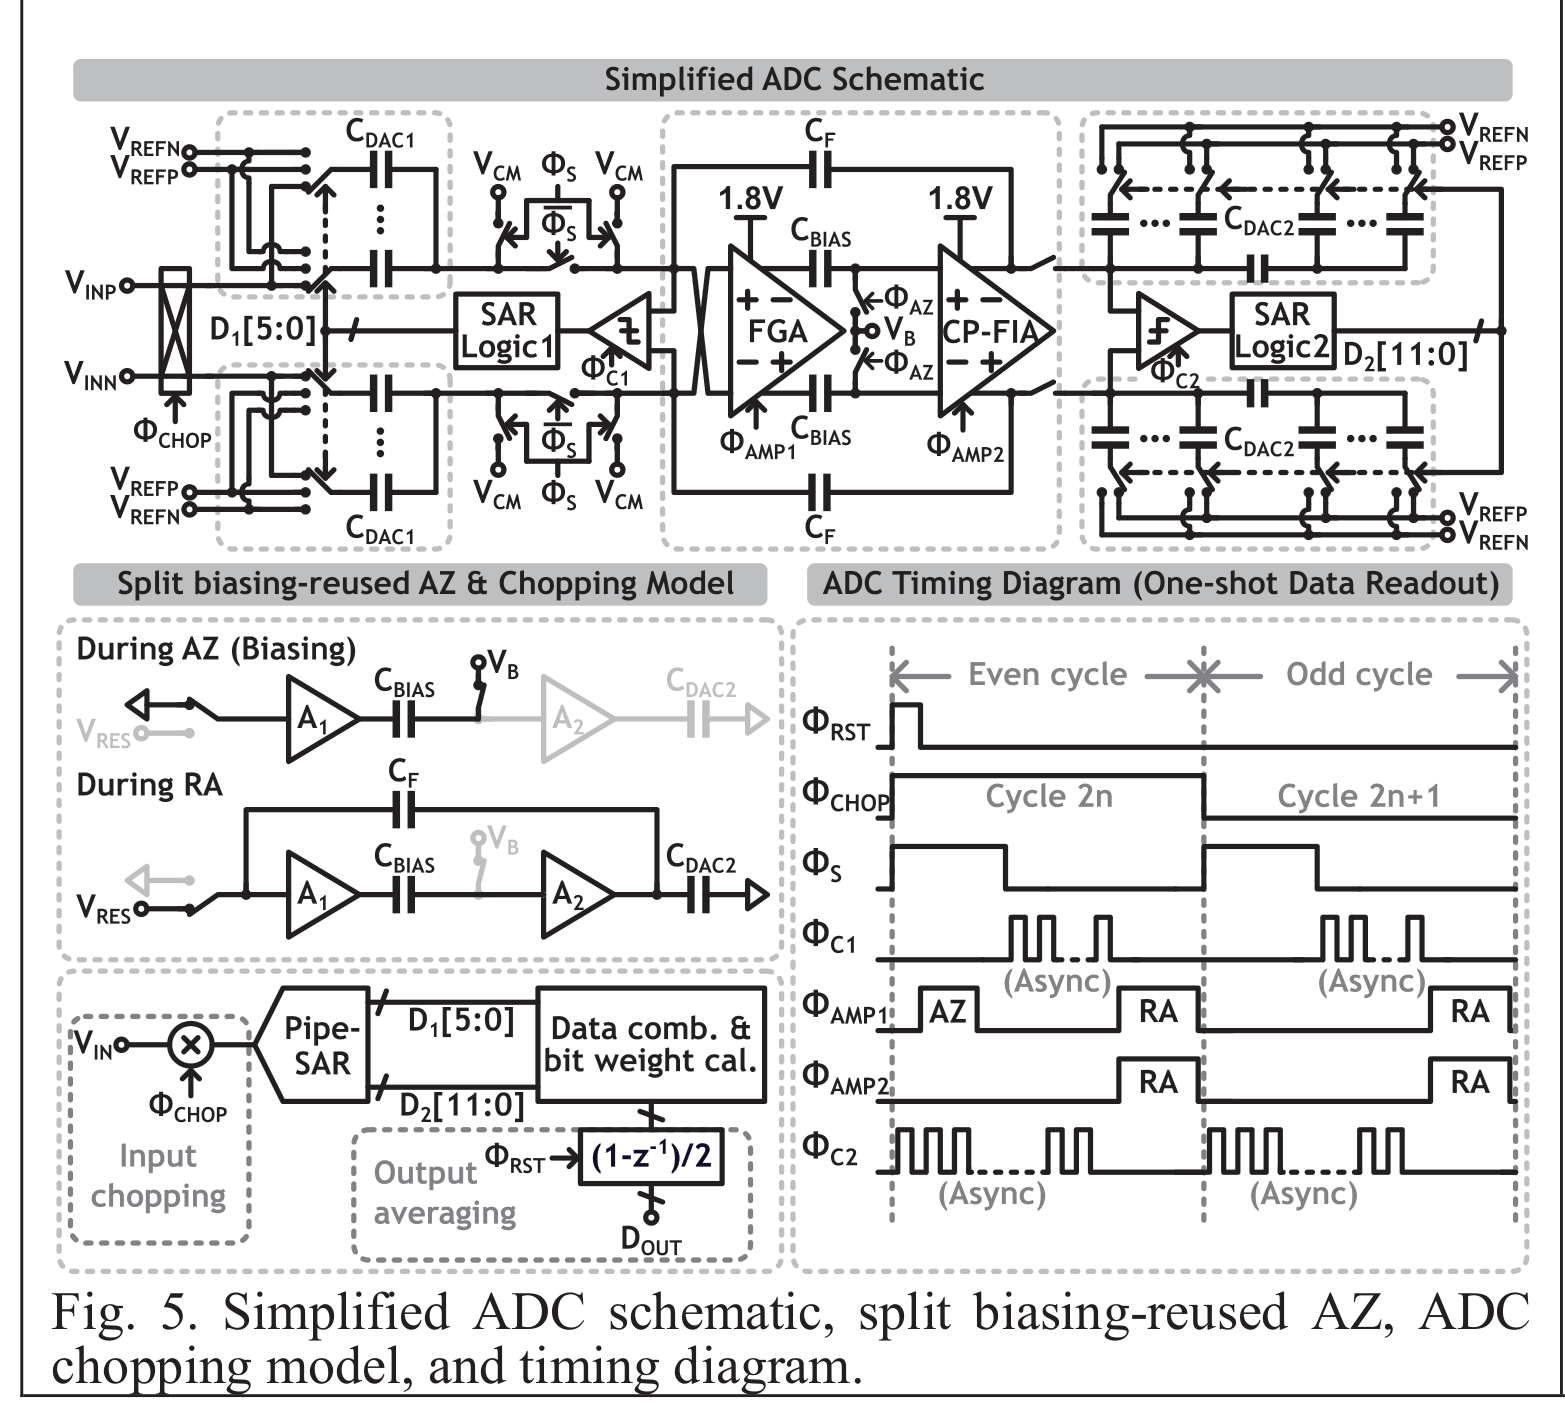
\includegraphics[width=125mm]{figures/source_caaz_fig5.png}
  \caption{Wang等VLSI 2025原论文Fig.5，PDF／印刷第2页：输入斩波、CBIAS、位权校正与输出处理}
  \label{fig:wang等vlsi-2025原论文fig-5-pdf-印刷第2页-输入斩波-cbias-位权校正与输出处理}
\end{figure}

该原型图的6位前级和FGA／CP-FIA只用于解释CAAZ位置；本项目仍保持ISSCC的9位交织前级。输入差分极性先由ΦCHOP切换，CBIAS位于RA内部。图左下顺序是输入换相$\to$ADC$\to$数据合并与位权校正$\to$输出处理。数字同学实现控制、元数据和重构／配对，不承担FGA、CP-FIA或保持开关的晶体管设计。

\textbf{与DEM／dither协作：}先在每笔原始斩波码域中完成该笔的位权重构与去扰，再解调配对。奇偶笔可以选不同物理片、不同DEM相位及不同扰动字，但每笔必须携带自己的实际mask。共享的是AZ代，不是切片、电容误差或扰动字。

\textbf{复现要求：}把捕获／保持请求和行为确认随样本ID对齐。样本域模型必须偶笔保存w、奇笔复用同一w或其保持误差版本；不能只发hold标志却每笔重抽AZ噪声。当前联合模型已按此构造。实际电路对接另行落实。本项目把dither定义在斩波后的码域，是需模拟签认的工程位置；若真实注入在斩波前，须重新推导符号与接口。


\clearpage
\section{技术说明：共享AZ怎样抵消噪声，哪些噪声不会消失}

\begin{figure}[H]
  \centering
  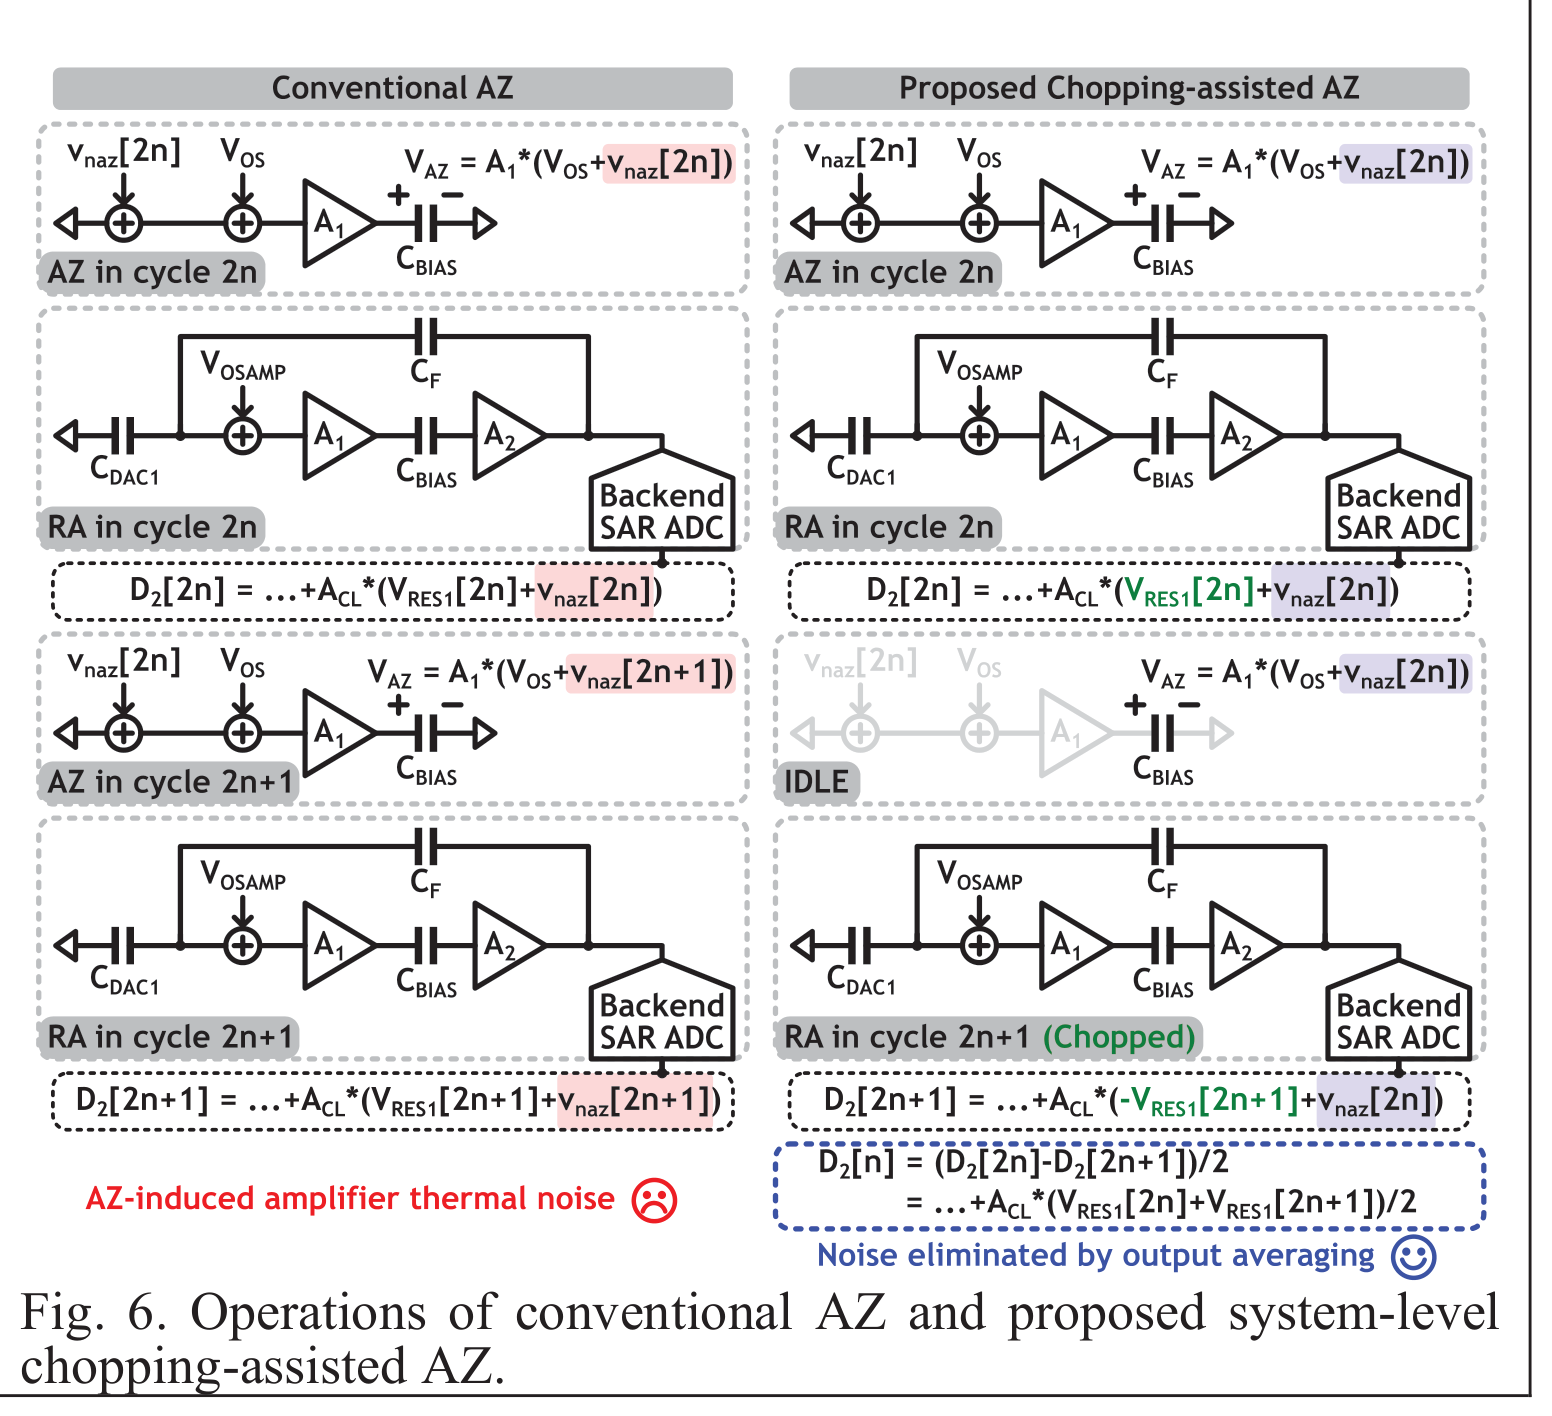
\includegraphics[width=120mm]{figures/source_caaz_fig6.png}
  \caption{北大原论文Fig.6，PDF／印刷第2页：偶周期捕获、奇周期保持，输入反相；©~2025 JSAP}
  \label{fig:北大原论文fig-6-pdf-印刷第2页-偶周期捕获-奇周期保持-输入反相-2025-jsap}
\end{figure}

论文PDF第1页Fig.6说明的原句为：

\begin{quote}
``AZ is only performed in the even cycle''
\end{quote}

原文还指出：

\begin{quote}
``two consecutive conversion results contain the same sampled noise''
\end{quote}

用输入等效量说明：z\_e=x\_e+a\_e w+u\_e，z\_o=--x\_o+a\_o h w+u\_o。其中w是同一份AZ噪声，h为保持比例，a\_e、a\_o为两相传递，u为独立误差。配对结果：

\begin{equation}
y=\frac{z_e-z_o}{2}=\frac{x_e+x_o}{2}+\frac{a_e-h a_o}{2}w+\frac{u_e-u_o}{2}.
\end{equation}

当h=1且a\_e=a\_o时，共享项抵消；独立噪声仍有方差$\sigma_u^2/2$。相邻笔相同的残余失调也能相消，时变失调／低频噪声只受到滤波抑制。增益不同、泄漏、重新捕获AZ或错绑代号都会留下残余。残余AZ标准差为|a\_e--h a\_o|σ\_w/2；参数须来自模拟条件或标明敏感性扫描。

\textbf{原文提出它的意义：}传统AZ会额外采入CBIAS热噪声；共享AZ配合信号换相，可以抵消这份新增噪声，而普通两笔平均只让独立噪声功率减半。论文第1页报告总热噪声改善4.3 dB，其中3 dB来自普通平均、额外1.3 dB来自AZ采样噪声抵消；应用针对低至中频输入，不是无代价提高任意宽带转换性能。


\clearpage
\section{技术说明：配对频响、整数舍入与CAAZ复现要求}

\begin{figure}[H]
  \centering
  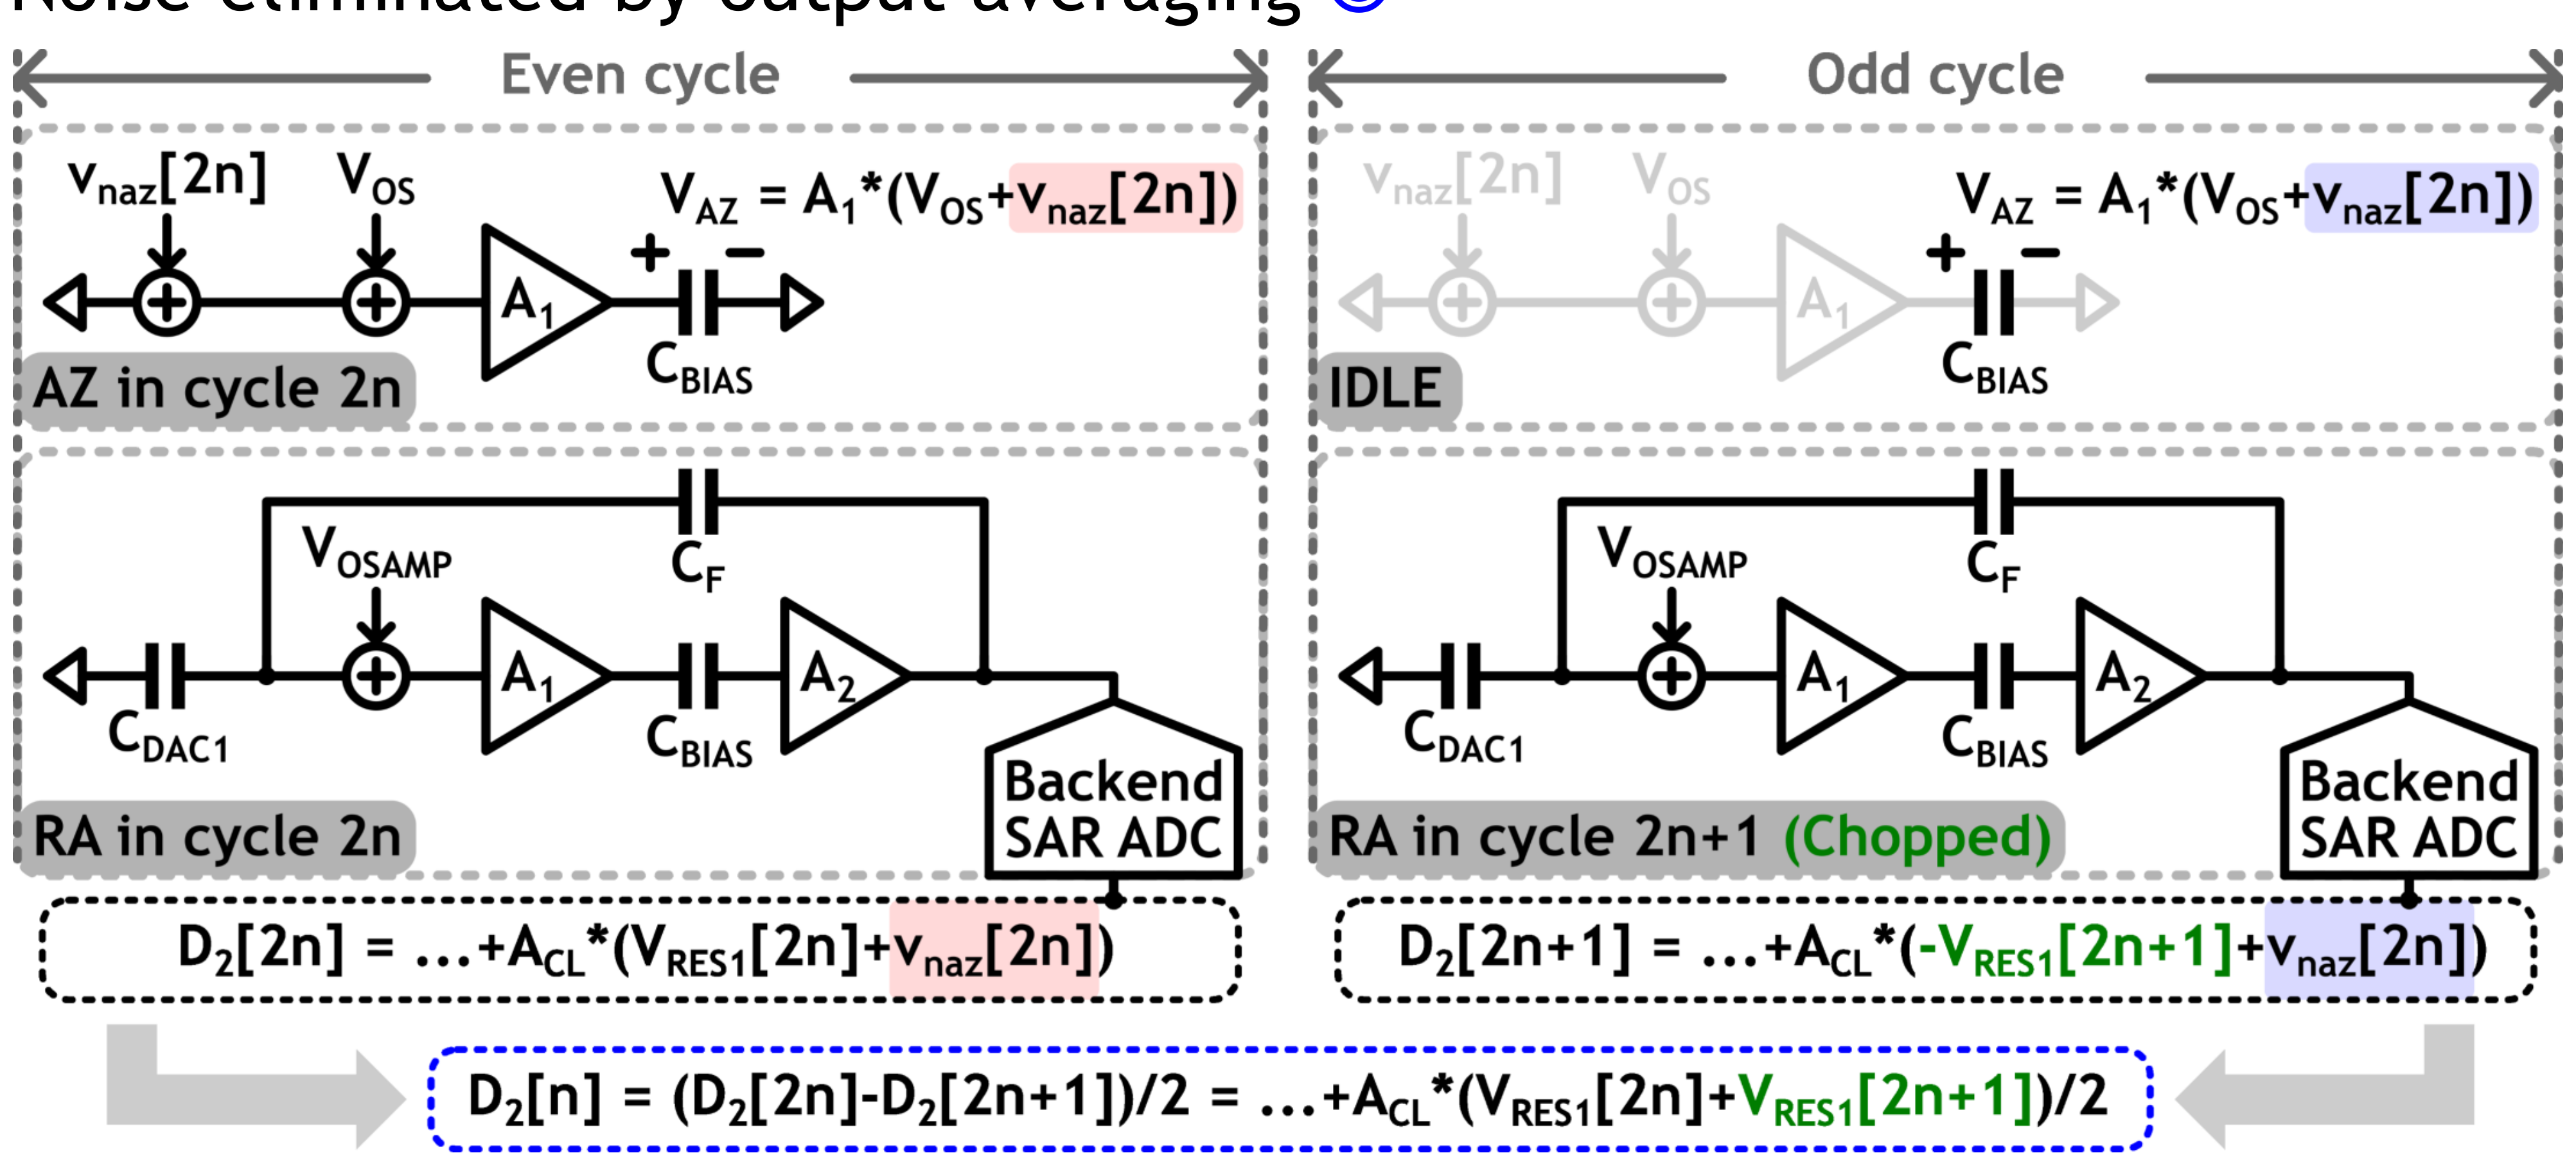
\includegraphics[width=146mm]{figures/source_caaz_slide35.png}
  \caption{北大讲稿PDF第35页、幻灯片34原图节选：同一噪声、相反信号与偶减奇；©~2025 JSAP}
  \label{fig:北大讲稿pdf第35页-幻灯片34原图节选-同一噪声-相反信号与偶减奇-2025-jsap}
\end{figure}

\textbf{数字直觉：}若偶数码1008、奇数码--992，二者包含同一+8误差，则差的一半为1000；若奇数误差只剩+6，结果变为1001。例子只解释共享与保持关系，不代表芯片噪声幅度。

\textbf{码宽与舍入：}当前caaz20\_pair保留21位有符号差d=e--o，范围$\pm$1,048,575，以半LSB解释；20位输出为floor(d/2)。d=--1时输出--1，同时保留精确--0.5 LSB差量。不能把浮点平均无条件当作RTL整数oracle。

\textbf{频响与带宽：}10 MS/s原始流的两点信号平均具有|cos(πf/10 MHz)|幅频响应，配对时间戳取两孔径中点，输出5 MS/s。工程例中1 MHz幅度约降0.44 dB，2.5 MHz约降3.01 dB；两点平均也不是完整抗混叠滤波器。因此CAAZ对照必须同输出速率、同带宽，分开报告普通平均与共享AZ的收益。

\textbf{速率定义：}原论文及讲稿标称转换速度6 MS/s，但未在已核对文字中单列内部原始码率与对外配对码率，不能擅自写成6$\to$3或12$\to$6。本工程明确采用非重叠10$\to$5，作为可选低噪声模式；旁路保持10。若最终输出必须10且CAAZ开启，需另定内部吞吐与时序，不能把当前5 MS/s结果算作10 MS/s输出目标完成。

\textbf{解调、滤波与抽取分开：}逐笔乘斩波极性是数字解调，本身不改变码率；差分／相关处理可以与解调融合。图中$ (1-z^{-1})/2 $的除2是幅度归一化，不是2:1抽取指令。当前代码只在合格奇数笔发布一对结果，才明确形成10$\to$5；不能仅凭原图的除2推断原文ADC码率减半。若研究全速逐笔解调／滤波，应另行验证，不用现有半速数据代替。

\textbf{测量的10$\times$平均：}讲稿PDF第38页、幻灯片37的Measured Spectrum写有64k-points,~10x averaging，这是谱测量设置，与CAAZ解调和输出抽取不同。常见功率谱平均可稳定谱底起伏，不等于时域每10码合成一码，也不自动提高ADC的SNDR 10 dB。原文未写明功率／幅度／复数平均类型；复现时须单列FFT点数、窗函数、平均方式及归一化，不能替作者补全或仅比较噪声底高度。

\textbf{复现要求：}先固定同一颗2\%／3\%池和冻结LMS，比较独立AZ、共享AZ、含保持误差，再改变DEM／dither开关验证协作。交保持扫描、误差谱、AZ代／极性时序和错绑负例；独立量化误差、动态建立和未去尽扰动不能算作``被CAAZ消掉''。原型6 MS/s与本项目10／5 MS/s分别记录，不搬用其SNDR数字作验收门槛。


% ----- end md -----
\end{document}
